\chapter{Extremal Kerr black hole}
\label{s:exk}

\minitoc

\section{Introduction}

The Kerr solution of the Einstein equation has been introduced in Sec.~\ref{s:ker:Kerr_solution};
it depends on two parameters: the mass $m > 0$ and the spin parameter
$a \geq 0$.
In Chaps.~\ref{s:ker}--\ref{s:gik}, we have considered the Kerr solution with $0<a<m$
and the case $a=0$ (Schwarzschild solution) has been treated in Chaps.~\ref{s:sch}--\ref{s:max}.
Here we focus on the case $a=m$, which is called the \emph{extremal Kerr spacetime}.
This corresponds to the highest value of $a$
for which the Kerr solution describes a black hole.
Indeed, for $a> m$, the Kerr metric is still an exact
solution of the vacuum Einstein equation (\ref{e:fra:vac_Einstein}), but it describes a \emph{naked singularity}\index{naked singularity} (cf. Sec.~\ref{s:max:naked_sing}):
the ring singularity is not hidden by any horizon to asymptotic observers.

The Kerr spacetime with $a=m$ is not just the maximally spinning black hole of the Kerr family.
As we going to see, it has important properties that are not
shared by Kerr spacetimes with $a<m$. In particular, the black hole event horizon is
\emph{degenerate}, in the sense defined in Sec.~\ref{s:neh:classif_KH}, i.e. it has a
vanishing surface gravity $\kappa$. Besides, there is no internal horizon
and the maximal analytic extension, to be constructed in Sec.~\ref{s:exk:max_extension}
below, is simpler than
that of the Kerr spacetime with $a<m$.
Another specific property of the extremal Kerr spacetime (actually related
to the degeneracy of the horizon)
regards the geometry near the horizon: it admits an enlarged
symmetry group, which is generated
by four independent Killing vectors,
instead of two for the geometry of the global solution.
This is called the \emph{NHEK} geometry (for \emph{near-horizon extremal Kerr})
and has received considerable attention in the recent literature. We shall
discuss it in Sec.~\ref{s:exk:NHEK}.


%%%%%%%%%%%%%%%%%%%%%%%%%%%%%%%%%%%%%%%%%%%%%%%%%%%%%%%%%%%%%%%%%%%%%%%%%%%%%%%

\section{Definition and basic properties}

\subsection{The extremal Kerr solution}

Let us consider the manifold $\R^2\times\SS^2$ described by
coordinates $(\ti, r, \th,\tph)$ such that $(\ti,r)$ cover $\R^2$
and $(\th,\tph)$ are standard spherical coordinates on $\SS^2$.
The \defin{extremal Kerr spacetime}\index{extremal!Kerr!spacetime}\index{Kerr!extremal -- spacetime}
of mass $m>0$ is defined as the pair $(\M, \w{g})$ where the manifold $\M$ is the following open subset of $\R^2\times\SS^2$:
\be \label{e:exk:def_M}
 \M := \R^2\times\SS^2 \setminus \ring
\ee
with
\be \label{e:exk:def_ring}
    \ring := \left\{ p \in \R^2\times\SS^2,
        \quad r(p) = 0 \ \mbox{and}\ \th(p) = \frac{\pi}{2} \right\} ,
\ee
and the metric $\w{g}$ has the following expression in terms of the coordinates
$(x^{\tilde{\alpha}}) = (\ti, r, \th,\tph)$:
\be \label{e:exk:metric_Kerr_3p1}
    \encadre{
    \begin{array}{ll}
   \w{g}  = &
    \displaystyle - \left( 1 - \frac{2m r}{\rho^2} \right)  \dd \ti^2
    + \frac{4m r}{\rho^2} \dd\ti\, \dd r
    - \frac{4 m^2  r \sin^2\th}{\rho^2} \,  \dd \ti\, \dd\tph \\[2ex]
    &\displaystyle  + \left( 1 + \frac{2m r}{\rho^2} \right) \dd r^2
     - 2 m \left( 1 + \frac{2m r}{\rho^2} \right) \sin^2\th \, \dd r\, \dd \tph \\[2ex]
    & \displaystyle + \rho^2 \dd \th^2
    + \left( r^2 + m^2 + \frac{2 m^3 r \sin^2\th}{\rho^2} \right)
    \sin^2\th \, \dd \tph^2 ,
    \end{array}
    }
\ee
with
\be
    \rho^2 := r^2 + m^2\cos^2\th .
\ee
In this context, the coordinates $(x^{\tilde{\alpha}}) = (\ti, r, \th,\tph)$
are called
\defin{Kerr coordinates}\index{Kerr!coordinates}
and we recognize in (\ref{e:exk:metric_Kerr_3p1}) the limit $a\to m$ of
expression (\ref{e:ker:metric_Kerr_3p1}) for the Kerr metric with $a< m$.

The metric (\ref{e:exk:metric_Kerr_3p1}) is regular
in all $\M$, since the components $g_{\tilde{\alpha}\tilde{\beta}}$ are singular only
for $\rho=0$, i.e. for $r=0$ and $\th=\pi/2$, which defines  the set $\ring$ that has precisely been excluded from $\M$ in
the definition (\ref{e:exk:def_M}). The Kretschmann curvature
invariant\index{Kretschmann scalar! of Kerr metric} $K := R_{\mu\nu\rho\sigma} R^{\mu\nu\rho\sigma}$
is given by Eq.~(\ref{e:ker:Kretschmann}) with $a=m$; it diverges for $\rho\to 0$. Therefore, as
for the Kerr spacetime with $a<m$ (cf. Sec.~\ref{s:ker:singularities}), we shall call $\ring$ the \defin{ring singularity}\index{ring!singularity}\index{singularity!ring --}
of the extremal Kerr spacetime. Note that, formally, it is not part of the spacetime manifold
$\M$ [cf. Eq.~(\ref{e:exk:def_M})].

Moreover, the Ricci tensor of the metric (\ref{e:exk:metric_Kerr_3p1}) is identically zero in all
$\M$ (see the notebook~\ref{s:sam:Kerr_extremal} for the computation). Hence, we have:

\begin{prop}[extremal Kerr metric as a solution of the vacuum Einstein equation]
The metric $\w{g}$ of the extremal Kerr spacetime is a solution of the
vacuum Einstein equation\index{Einstein!equation!vacuum --}\index{vacuum!Einstein equation} $\w{R}=0$ [Eq.~(\ref{e:fra:vac_Einstein})].
\end{prop}

The inverse metric is
\be \label{e:exk:inv_met_3p1}
    g^{\tilde{\alpha}\tilde{\beta}} = \left(
    \begin{array}{cccc}
    - \left( 1 + \frac{2m r}{\rho^2} \right) & \frac{2m r}{\rho^2} & 0 & 0 \\[1ex]
    \frac{2m r}{\rho^2} & \frac{(r-m)^2}{\rho^2} & 0 & \frac{m}{\rho^2} \\[1ex]
    0 & 0 &\frac{1}{\rho^2} & 0 \\[1ex]
    0 & \frac{m}{\rho^2} & 0 & \frac{1}{\rho^2\sin^2\th}
    \end{array}
    \right) .
\ee


\subsection{Boyer-Lindquist coordinates}

For $a<m$, the Kerr manifold $\M$ has been split in three open regions,
$\M_{\rm I}$, $\M_{\rm II}$ and $\M_{\rm III}$,  separated by the two Killing
horizons $\Hor$ and $\Hor_{\rm in}$
[cf. Eqs.~(\ref{e:ker:def_M_Kerr_spacetime}) and (\ref{e:ker:def_M_BL})].
Since $\Hor$ was defined by $r=r_+:=m + \sqrt{m^2 - a^2}$ [Eq.~(\ref{e:ker:def_H})]
and $\Hor_{\rm in}$
by $r=r_-:=m - \sqrt{m^2 - a^2}$ [Eq.~\ref{e:ker:def_H_in})],
we notice that
$r_+ = r_- = m$ in the limit $a\to m$.
This implies that $\Hor$ and $\Hor_{\rm in}$ coincide when $a\to m$ and the region
$\M_{\rm II}$, which is bounded by $\Hor$ and $\Hor_{\rm in}$, disappears.
Accordingly, we shall split the extremal Kerr manifold $\M$ in two open regions only,
$\M_{\rm I}$ and $\M_{\rm III}$, separated by a single hypersurface $\Hor$:
\be
    \encadre{\M = \M_{\rm I} \cup \Hor \cup \M_{\rm III} },
\ee
with
\begin{subequations}
\begin{align}
    \M_{\rm I} & := \left\{ p \in \M, \quad r(p) > m \right\} \\
    \Hor & := \left\{ p \in \M, \quad r(p) = m \right\} \label{e:exk:def_H}\\
    \M_{\rm III} & := \left\{ p \in \M, \quad r(p) < m \right\} .
\end{align}
\end{subequations}
\begin{remark}
We are using the notation $\M_{\rm III}$ for the ``second'' region, and not $\M_{\rm II}$,
to be consistent with Chaps.~\ref{s:ker}--\ref{s:gik}, i.e. with
the limit $a\to m$ of the results obtained in these chapters.
\end{remark}
The quadratic polynomial in $r$ introduced in Chap.~\ref{s:ker},
$\Delta=r^2 - 2 m r + a^2 = (r - r_+)(r - r_-)$, reduces to $\Delta = (r - m)^2$
in the limit $a\to m$. Its double root, $r=m$, defines the hypersurface $\Hor$.


In the region $\M_{\rm BL}:= \M \setminus \Hor = \M_{\rm I} \cup \M_{\rm III}$, one may introduce
the \defin{Boyer-Lindquist coordinates}\index{Boyer-Lindquist coordinates}
$(t,r,\th,\ph)$ such that $(r,\th)$ are the same coordinates as in
Kerr coordinates, while $t$ and $\ph$ are related to the Kerr coordinates
$\ti$, $r$ and $\tph$ by
\begin{subequations}
\label{e:exk:3p1_Kerr_to_BL}
\begin{align}
    t & = \ti +  \frac{2m^2}{r - m} - 2m \ln \left| \frac{r - m}{m} \right|
            \label{e:exk:3p1_Kerr_to_BL_t} \\
    \ph & = \tph + \frac{m}{r - m} . \label{e:exk:3p1_Kerr_to_BL_ph}
\end{align}
\end{subequations}
Differentiating these relations leads to
\be \label{e:exk:dt_dph}
    \dd \ti = \dd t  + \frac{2m r}{(r- m)^2} \, \dd r
    \qand
    \dd \tph = \dd \ph + \frac{m}{(r - m)^2 } \, \dd r .
\ee
\begin{remark}
The differential relations (\ref{e:exk:dt_dph}) can be obtained immediately
by substituting $a$ by $m$ in relations (\ref{e:ker:Kerr_3p1_BL}). However, to get the integrated
relations (\ref{e:exk:3p1_Kerr_to_BL}) from their $a<m$ counterpart
(\ref{e:ker:Kerr_3p1_BL_int}), one must perform an expansion in $\veps := \sqrt{m^2 - a^2}/m$,
taking into account that $r_\pm = m(1\pm\veps)$. One obtains then
(\ref{e:exk:3p1_Kerr_to_BL_t})
up to the additive constant $(2\ln 2) m$, while (\ref{e:exk:3p1_Kerr_to_BL_ph}) is recovered in the same form.
\end{remark}
It follows from the transformations (\ref{e:exk:3p1_Kerr_to_BL}) that
the Boyer-Lindquist coordinate frame $(\wpar_\alpha)$ and the Kerr coordinate frame $(\wpar_{\tilde{\alpha}})$ are related by\footnote{See also the limit $a\to m$ of Eq.~(\ref{e:ker:frame_Kerr3p1_BL}).}
\begin{subequations}
\label{e:exk:frame_BL_Kerr3p1}
\begin{align}
    & \wpar_t  = \wpar_\ti  \\
    & \wpar_r = \wpar_{\tilde r} + \frac{2mr}{(r-m)^2} \wpar_\ti
                        + \frac{m}{(r-m)^2} \wpar_\tph \\
    & \wpar_\th = \wpar_\th \\
    & \wpar_\ph = \wpar_{\tph} .
\end{align}
\end{subequations}

\begin{remark}
As in Chap.~\ref{s:ker}, we have denoted by $\wpar_{\tilde r}$ the second vector of the
coordinate frame associated to the Kerr coordinates
$(x^{\tilde{\alpha}}) = (\ti, r, \th,\tph)$, in order to distinguish it from
the coordinate vector
$\wpar_r$ of the Boyer-Lindquist coordinates
$(x^\alpha) = (t,r,\th,\ph)$.
\end{remark}

\begin{figure}
\centerline{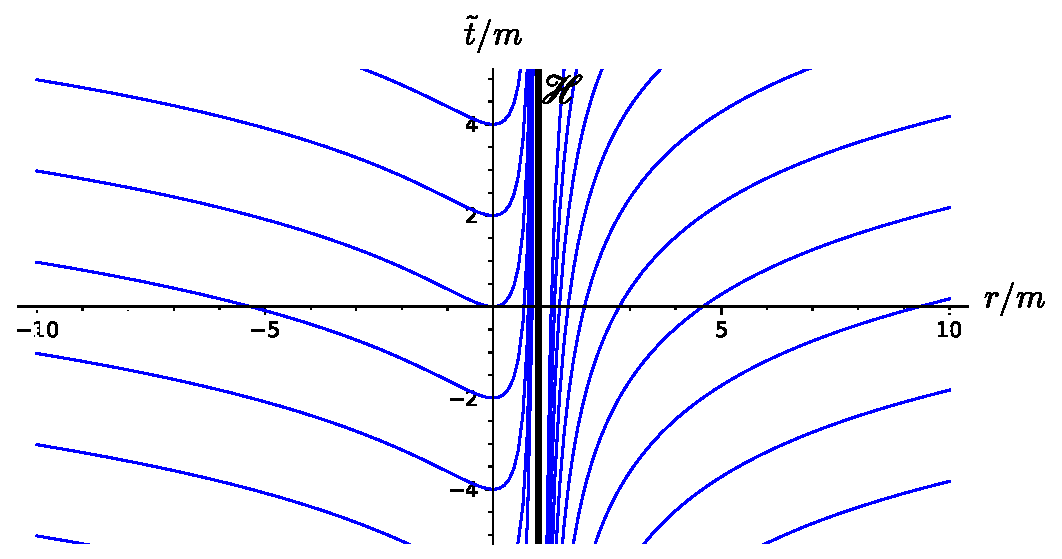
\includegraphics[width=0.7\textwidth]{exk_BL_slicing.pdf}}
\caption[]{\label{f:exk:BL_slicing} \footnotesize
Trace of the hypersurfaces of constant Boyer-Lindquist time $t$ in the plane
$(\tilde{t}, r)$.
\textsl{[Figure generated by the notebook \ref{s:sam:Kerr_extremal}]}
}
\end{figure}

The metric components $(g_{\alpha\beta})$ with respect to the Boyer-Lindquist coordinates $(x^\alpha) = (t,r,\th,\ph)$ are given by
\be \label{e:exk:metric_BL}
    \encadre{
    \begin{array}{ll}
    \w{g} = &
    \displaystyle - \left( 1 - \frac{2m r}{\rho^2} \right) \, \dd t^2
    - \frac{4 m^2  r \sin^2\th}{\rho^2} \,  \dd t\, \dd\ph
    + \frac{\rho^2}{(r-m)^2} \, \dd r^2  \\[2ex]
    & \displaystyle + \rho^2 \dd \th^2
    + \left( r^2 + m^2 + \frac{2 m^3 r \sin^2\th}{\rho^2} \right)
    \sin^2\th \, \dd \ph^2 .
    \end{array}
    }
\ee
This expression can be obtained either by taking the limit $a\to m$ of Eq.~(\ref{e:ker:metric_BL})
or by using (\ref{e:exk:dt_dph}) to substitute $\dd\ti$ and $\dd\tph$ in Eq.~(\ref{e:exk:metric_Kerr_3p1}).
We note that $g_{rr}\to +\infty$ when $r\to m$, which reflects the singularity of Boyer-Lindquist
coordinates on $\Hor$ and explains why the latter was excluded in the definition
of $\M_{\rm BL}$. This singularity is clearly apparent in the coordinate transformations
(\ref{e:exk:3p1_Kerr_to_BL}), as well as in the spacetime slicing by the
hypersurfaces $t=\mathrm{const}$ depicted in Fig.~\ref{f:exk:BL_slicing}: the slices accumulate
onto $\Hor$, without crossing it, so that the points on $\Hor$ do not belong to any
hypersurface $t=\mathrm{const}$. That the $t=\mathrm{const}$ hypersurfaces do not provide a
regular slicing of the extremal Kerr spacetime $(\M,\w{g})$ is also manifest on
the Carter-Penrose diagram shown in Fig.~\ref{f:exk:CPdiag_BL}.

The Boyer-Lindquist components of the
inverse metric $\w{g}^{-1}$ are
\be \label{e:exk:inv_met_BL}
    g^{\alpha\beta} = \left(
    \begin{array}{cccc}
    - \frac{1}{(r-m)^2}
    \left( r^2 + m^2 + \frac{2 m^3 r \sin^2\th}{\rho^2} \right)
     & 0 & 0 & -\frac{2 m^2 r}{\rho^2 (r-m)^2} \\[1ex]
    0 & \frac{(r-m)^2}{\rho^2} & 0 & 0 \\[1ex]
    0 & 0 &\frac{1}{\rho^2} & 0 \\[1ex]
    -\frac{2 m^2 r}{\rho^2 (r-m)^2} & 0 & 0 &
    \frac{1}{(r-m)^2\sin^2\th}\left(1 - \frac{2 m r}{\rho^2} \right)
    \end{array}
    \right) .
\ee
They can also be obtained by taking the limit $a\to m$ of Eq.~(\ref{e:ker:inv_met_BL}).

\subsection{Symmetries}

The extremal Kerr metric (\ref{e:exk:metric_Kerr_3p1}) is stationary\footnote{Cf.
Sec.~\ref{s:sta:def_station} for the definition of \emph{stationary} and some discussion
about the terminology.} and axisymmetric. The corresponding isometry group is
$\R\times\mathrm{SO}(2)\simeq \R\times\mathrm{U}(1)$ and is generated
by two commuting Killing vectors $\w{\xi}$ and $\w{\eta}$. Both the Kerr coordinates and
the Boyer-Lindquist ones are adapted to the spacetime symmetries, i.e. $(\ti,\tph)$ and
$(t,\ph)$ are ignorable coordinates, as it is clear from the
metric components (\ref{e:exk:metric_Kerr_3p1})
and (\ref{e:exk:metric_BL}). Accordingly, one can normalize the Killing vectors so that
\be \label{e:exk:Killing_vectors}
    \encadre{\w{\xi} = \wpar_{\ti} = \wpar_t}
    \qand
    \encadre{\w{\eta} = \wpar_{\tph} = \wpar_\ph} .
\ee

\begin{figure}
\centerline{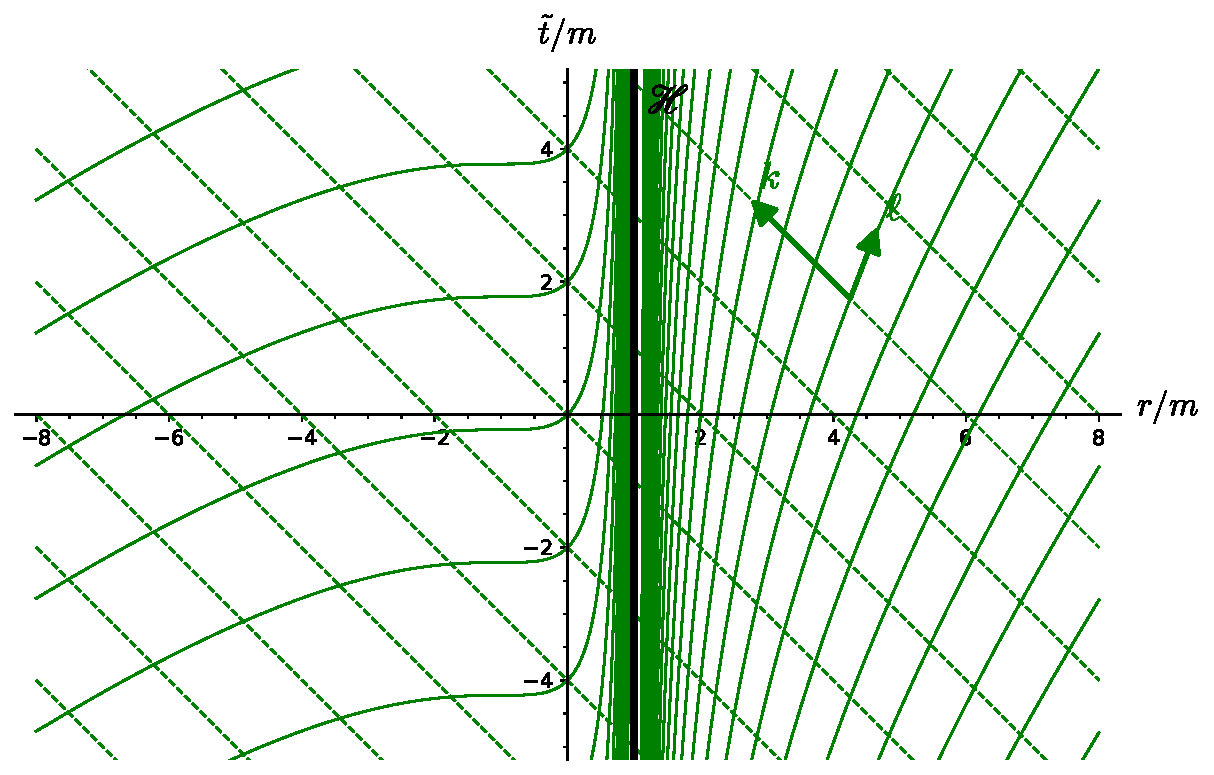
\includegraphics[width=0.8\textwidth]{exk_princ_null_geod.pdf}}
\caption[]{\label{f:exk:princ_null_geod} \footnotesize
Trace of the principal null geodesics in the plane
$(\tilde{t}, r)$. The dashed lines correspond to the
ingoing principal null geodesics $\Li^{\rm in}_{(v,\th,\tph)}$
and the solid curves to the
outgoing principal null geodesics $\Li^{\rm out,I}_{(u,\th,\tilde{\tph})}$
for $r>m$ and $\Li^{\rm out,III}_{(u,\th,\tilde{\tph})}$ for $r<m$.
\textsl{[Figure generated by the notebook \ref{s:sam:Kerr_extremal}]}
}
\end{figure}



\subsection{Principal null geodesics} \label{s:exk:princ_null_geod}

As discussed in Sec.~\ref{s:ker:principal_geod}, the Kerr spacetime is
endowed with two congruences of null geodesics tied to
the spacetime structure, as described by the Weyl conformal curvature tensor.
All the results of Sec.~\ref{s:ker:principal_geod} remain valid at the limit $a\to m$.
We can summarize them as follows:
\begin{prop}[principal null geodesics of the extremal Kerr spacetime]
\begin{itemize}
\item The \defin{ingoing principal null geodesics} are the curves
\be
    \Li^{\rm in}_{(v,\th,\tph)}:\quad
        (v,\th,\tph) = \mathrm{const} \in \R\times[0,\pi]\times[0,2\pi), %]
\ee
where $v$ is the Kerr advanced time:
\be \label{e:exk:def_v}
    v := \ti + r = t  + r - \frac{2m^2}{r -m} + 2m\ln\left| \frac{r - m}{m} \right|.
\ee
Along any geodesic $\Li^{\rm in}_{(v,\th,\tph)}$, $-r$ is an affine parameter increasing towards the future;
the corresponding tangent vector is
\begin{subequations}
\begin{align}
 \w{k} & = \wpar_{\ti} - \wpar_{\tilde{r}} \label{e:exk:k_3p1_Kerr}\\
 \w{k} & = \frac{r^2 + m^2}{(r - m)^2} \, \wpar_t
            - \wpar_r + \frac{m}{(r - m)^2} \, \wpar_\ph
            \quad \mbox{in}\ \M\setminus\Hor .  \label{e:exk:k_BL}
\end{align}
\end{subequations}
\item The \defin{outgoing principal null geodesics} are the curves
\begin{subequations}
\begin{align}
  \mbox{in}\ \M_{\rm I} :&\quad \Li^{\rm out, I}_{(u,\th,\tilde{\tph})}:
    \quad   (u,\th,\tilde{\tph}) = \mathrm{const} \in \R\times[0,\pi]\times[0,2\pi), \\ %]
  \mbox{in}\ \M_{\rm III}:&\quad \Li^{\rm out, III}_{(u,\th,\tilde{\tph})}:
    \quad   (u,\th,\tilde{\tph}) = \mathrm{const} \in \R\times[0,\pi]\times[0,2\pi), \\ %]
 \mbox{on}\  \Hor: &\quad \Li^{{\rm out},\Hor}_{(\th,\psi)}:
    \quad  (\th,\psi) = \mathrm{const} \in [0,\pi]\times[0,2\pi),  %]
\end{align}
\end{subequations}
where $u$ is the Kerr retarded time:
\be \label{e:exk:def_u}
    u := \ti - r + \frac{4 m^2}{r - m} - 4 m \ln \left| \frac{r - m}{m} \right|
      = t  - r + \frac{2m^2}{r -m} - 2m\ln\left| \frac{r - m}{m} \right|
\ee
and $\tilde{\tph}$ and $\psi$ are defined by
\be \label{e:exk:def_ttph}
    \tilde{\tph} := \tph + \frac{2m}{r -m} = \ph + \frac{m}{r - m}
\ee
and
\be \label{e:exk:psi_tph_ti}
    \psi := \tph - \frac{\ti}{2m} .
\ee
Along the geodesics $\Li^{\rm out, I}_{(u,\th,\tilde{\tph})}$ and $\Li^{\rm out, III}_{(u,\th,\tilde{\tph})}$,
$r$ is an affine parameter increasing towards the future,
while along $\Li^{{\rm out},\Hor}_{(\th,\psi)}$, such an affine parameter is $\ti$. The tangent vector $\wl$ to the outgoing principal null geodesics
that coincides with the Killing vector $\w{\xi} + (2m)^{-1} \w{\eta}$ on $\Hor$ is
\begin{subequations}
\begin{align}
 \wl & = \frac{(r + m)^2}{2(r^2 + m^2)}\, \wpar_{\ti}
  + \frac{(r - m)^2}{2(r^2 + m^2)} \,  \wpar_{\tilde{r}}
  + \frac{m}{r^2 + m^2} \, \wpar_{\tph} \label{e:exk:ell_3p1_Kerr}\\
 \wl & =  \frac{1}{2}\, \wpar_t
            + \frac{(r - m)^2}{2(r^2 + m^2)} \,  \wpar_r
            + \frac{m}{2(r^2 + m^2)} \, \wpar_\ph
            \quad \mbox{in}\ \M\setminus\Hor . \label{e:exk:ell_BL}
\end{align}
\end{subequations}
\end{itemize}
\end{prop}
\begin{proof}
The second equality in Eq.~(\ref{e:exk:def_v}) follows from Eq.~(\ref{e:exk:3p1_Kerr_to_BL_t}).
Equation~(\ref{e:exk:k_BL}) follows from Eq.~(\ref{e:exk:k_3p1_Kerr}) via Eq.~(\ref{e:exk:frame_BL_Kerr3p1}).
Equations~(\ref{e:exk:def_u}) and (\ref{e:exk:def_ttph}) are the integrated version of the system (\ref{e:ker:out_Kerr_Kerr_3p1}) with $a=m$. Equations~(\ref{e:exk:psi_tph_ti}), (\ref{e:exk:ell_3p1_Kerr})
and (\ref{e:exk:ell_BL}) are the $a=m$ versions of respectively
Eqs.~(\ref{e:ker:psi_tph_ti}), (\ref{e:ker:def_ell_outgoing}) and (\ref{e:ker:ell_BL}).
All the other statements follow from the limit $a\to m$ of results of Sec.~\ref{s:ker:principal_geod},
except for $\ti$ being an affine parameter along $\Li^{{\rm out},\Hor}_{(\th,\psi)}$, which
is peculiar to the extremal Kerr horizon and will
be proven in Sec.~\ref{s:exk:horizon}.
\end{proof}

The principal null geodesic congruences are depicted in terms of the $(\ti, r)$
coordinates in Fig.~\ref{f:exk:princ_null_geod}. Note that the outgoing geodesics
$\Li^{\rm out, I}_{(u,\th,\tilde{\tph})}$ and $\Li^{\rm out, III}_{(u,\th,\tilde{\tph})}$
tend to become tangent to $\Hor$ for $r\to m$; this agrees with $\Hor$ being
generated by some members of the outgoing principal null congruence, namely the geodesics
$\Li^{{\rm out},\Hor}_{(\th,\psi)}$, as we shall see in details in the next subsection.
Another view of the principal null geodesics is provided by the Carter-Penrose
diagram of $(\M,\w{g})$ shown in Fig.~\ref{f:exk:CPdiag_Kerr}, in which both
families of geodesics appear as straight lines.

\subsection{The degenerate horizon} \label{s:exk:horizon}

$\Hor$ is the hypersurface of $\M$ defined by $r=m$ [Eq.~(\ref{e:exk:def_H})]. Given
that the component $g^{rr} = (r - m)^2/\rho^2$ of the inverse metric with respect to Kerr coordinates
[Eq.~(\ref{e:exk:inv_met_3p1})] vanishes at $r=m$, we have
$g^{\tilde{\mu}\tilde{\nu}} \partial_{\tilde{\mu}} r \partial_{\tilde{\nu}} r = 0$ on $\Hor$,
which implies that the gradient $\vw{\nabla} r$
is a null vector there and that $\Hor$ is a null hypersurface.
Moreover, since the components of $\vw{\nabla} r$ are $\nabla^{\tilde{\alpha}} r = g^{\tilde{\alpha}r}$,
we read on Eq.~(\ref{e:exk:inv_met_3p1}) that
\be
    \vw{\nabla} r \equalH \frac{2m^2}{\rho^2} \wpar_{\ti} + \frac{m}{\rho^2} \wpar_{\tph}
        \equalH \frac{2 m^2}{\rho^2} \w{\chi} ,
\ee
where $\w{\chi}$ is the Killing vector field
\be \label{e:exk:def_chi}
    \encadre{\w{\chi} := \w{\xi} + \Omega_{\Hor} \w{\eta} },
    \qquad\mbox{with}\quad \encadre{\Omega_{\Hor} := \frac{1}{2m} }.
\ee
It follows immediately that $\Hor$ is a \emph{Killing horizon}, i.e. a null hypersurface
that admits a Killing vector as null normal (cf. Sec.~\ref{s:neh:def_Killing_hor}).

From expression~(\ref{e:exk:ell_3p1_Kerr}) for $\wl$, we have immediately
\be \label{e:exk:ell_chi_on_H}
    \wl \equalH \w{\chi} .
\ee
This means that the null generators of $\Hor$ are the outgoing principal null
geodesics $\Li^{{\rm out},\Hor}_{(\th,\psi)}$.

The \emph{surface gravity}\index{surface!gravity} $\kappa$ of the Killing horizon $\Hor$
has been defined in Sec.~\ref{s:neh:zeroth_law} as the non-affinity coefficient of the Killing-vector normal $\w{\chi}$ to $\Hor$:
$\wnab_{\w{\chi}}\, \w{\chi} \equalH \kappa \, \w{\chi}$ [Eq.~(\ref{e:neh:xi_nab_xi_kappa})].
Given the identity (\ref{e:exk:ell_chi_on_H}), $\kappa$ coincides with the value on $\Hor$ of the
non-affinity coefficient $\kappa_{\wl}$ of the tangent $\wl$ to the outgoing principal null
geodesics: $\wnab_{\wl}\, \wl = \kappa_{\wl}\, \wl$. A direct computation (cf. the notebook~\ref{s:sam:Kerr_extremal}) reveals that
\be
    \kappa_{\wl} = m \frac{r^2 - m^2}{(r^2 + m^2)^2} .
\ee
In particular, $\kappa_{\wl}$ vanishes for $r=m$, i.e. on $\Hor$.
Hence $\kappa = \left. \kappa_{\wl} \right| _{\Hor}$ leads to\footnote{The vanishing of $\kappa$ can also be obtained
by taking the limit $a\to m$ of expression (\ref{e:ker:kappa_m_a}), which has been derived for $a<m$.}
\be
    \encadre{\kappa = 0 } .
\ee
According to the classification introduced in Sec.~\ref{s:neh:classif_KH}, it follows
that $\Hor$ is a \emph{degenerate Killing horizon}\index{degenerate!Killing horizon}\index{Killing!horizon!degenerate --}.
The vanishing of the non-affinity coefficient $\kappa$ means that $\wl$ is a geodesic vector\index{geodesic!vector}
on $\Hor$, and not only a pregeodesic\index{pregeodesic!vector field}  one (cf. Remark~\ref{r:fra:geodesic_vector} in Sec.~\ref{s:fra:geod_motion}). Equivalently, at any given point $p\in\Hor$,
$\wl$ is the tangent vector associated to
an affine parameter $\lambda$ of the null geodesic $\Li^{{\rm out},\Hor}_{(\th,\psi)}$ through $p$.
Moreover, the affine parameter $\lambda$ coincides with $\ti$,
up to some additive constant. Indeed,
Eqs.~(\ref{e:exk:ell_chi_on_H}) and (\ref{e:exk:def_chi}) imply
\[
     \ell^{\ti} = \derd{\ti}{\lambda} = \chi^{\ti} = 1 ,
\]
from which $\lambda = \ti + \mathrm{const}$.
Since the range of $\ti$ is $(-\infty, +\infty)$, we conclude that
$\Li^{{\rm out},\Hor}_{(\th,\psi)}$ is a \emph{complete} geodesic. This constrasts
with the null generators of a non-degenerate Killing horizon, which are
incomplete, as shown in Sec.~\ref{s:sta:non-degenerate_KH}.

Let us summarize the results obtained above:
\begin{prop}[$\Hor$ as a degenerate Killing horizon]
\label{p:exk:H_degenerate_KH}
In the extremal Kerr spacetime, the hypersurface $\Hor$ defined
by $r=m$ is a degenerate Killing horizon.
Its generators are the outgoing principal null geodesics
$\Li^{{\rm out},\Hor}_{(\th,\psi)}$, which are complete geodesics
and which admit the Kerr coordinate
$\ti$ as an affine parameter. The tangent vector associated to this affine
parameter is the Killing vector $\w{\chi} = \w{\xi} + \Omega_{\Hor} \w{\eta}$
[Eq.~(\ref{e:exk:def_chi})], which coincides on $\Hor$ with the tangent
vector $\wl$ to the outgoing principal null congruence.
\end{prop}

\subsection{Black hole character} \label{s:exk:bhole_char}

As a Killing horizon, $\Hor$ is a null hypersurface and thus a one-way membrane
(cf. Sec.~\ref{s:def:hor_as_null}).
Since the ingoing principal null geodesics $\Li^{\rm in}_{(v,\th,\tph)}$
cross it from $\M_{\rm I}$ to $\M_{\rm III}$ (cf. Fig.~\ref{f:exk:princ_null_geod}),
we conclude that no (massive or null) particle can cross $\Hor$ from $\M_{\rm III}$
to $\M_{\rm I}$.
In order to show that $\Hor$ is actually a black hole event horizon,
it suffices to proceed as for the $a<m$ case treated in Sec.~\ref{s:ker:event_hor}.
We shall not repeat the argument here (which is based on the
asymptotics of Kerr spacetime being that of Schwarzschild spacetime --- a property
that holds for the extremal Kerr spacetime as well) and jump directly to the conclusion:

\begin{prop}[black hole region in the extremal Kerr spacetime]
The extremal Kerr spacetime $(\M, \w{g})$ can be endowed with a conformal
completion at null infinity such that the future and past null infinities $\scri^+$
and $\scri^-$ are located at the boundary of $\M_{\rm I}$. The region $\M_{\rm III}$ is
then the interior of a black hole, the event horizon of which is
the Killing horizon $\Hor$.
\end{prop}

The future null infinity $\scri^+$ and the past null infinity $\scri^-$
relative to $\M_{\rm I}$ are depicted in the Carter-Penrose diagram of
Figs.~\ref{f:exk:CPdiag_Kerr} -\ref{f:exk:CPdiag_BL}. In this diagram,
it is clear that $\M_{\rm III}$ is a black hole region for $\M_{\rm I}$
and that $\Hor$ is the corresponding event horizon.

\begin{figure}
\centerline{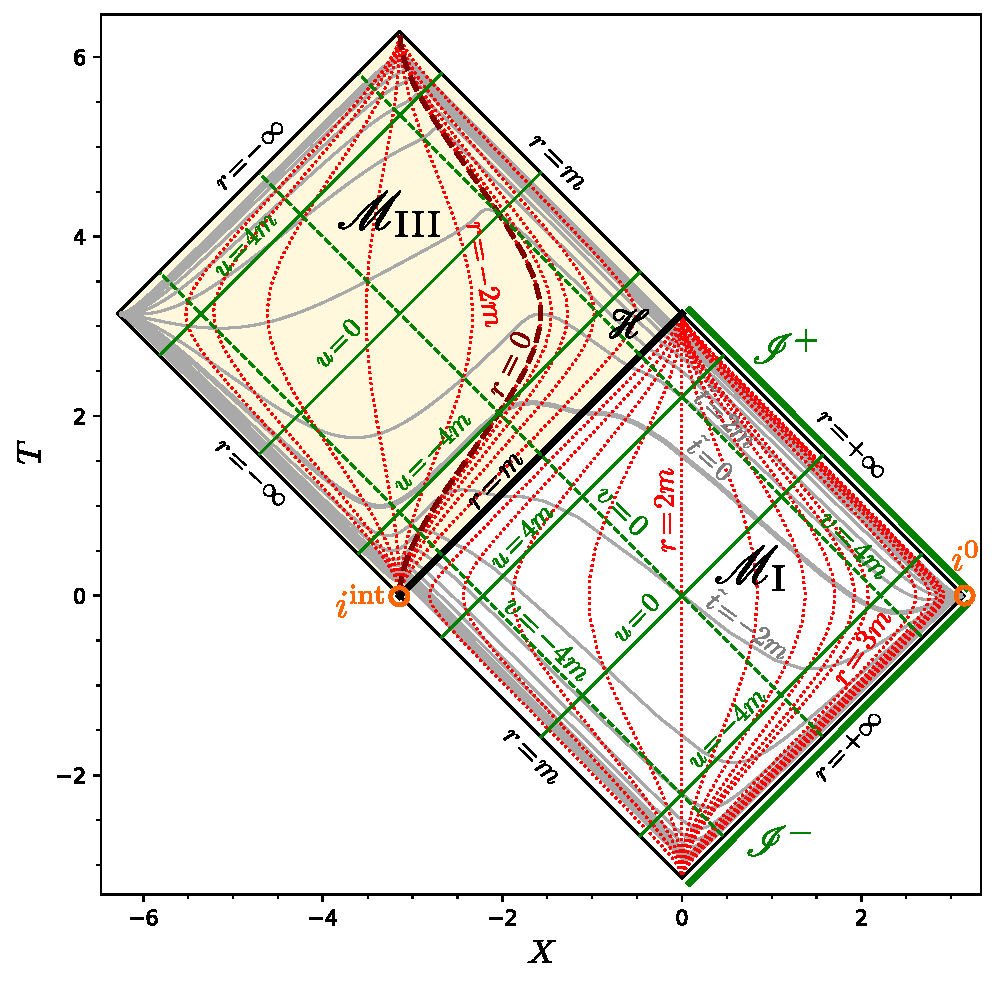
\includegraphics[width=0.8\textwidth]{exk_CPdiag_Kerr.pdf}}
\caption[]{\label{f:exk:CPdiag_Kerr} \footnotesize
Carter-Penrose diagram of the extremal Kerr spacetime $(\M,\w{g})$
constructed via the projection
map $\Pi:\ \M \to \R^2$,  $(\ti,r,\th,\tph)\mapsto (T, X)$
defined by Eqs.~(\ref{e:exk:projection_M})-(\ref{e:exk:def_T0_X0}).
The grey curves represent hypersurfaces $\ti=\mathrm{const}$, with
$\ti\in[-20 m, 20 m]$ and
the increment $\delta\ti = 2 m$ between two successive hypersurfaces.
The hypersurface $\ti=0$ is singled out by a larger thickness.
The red dotted curves represent hypersurfaces $r=\mathrm{const}$,
with the increment $\delta r$ between two successive hypersurfaces being
$\delta r = 2m$ for $r<0$ and $r> 3m$ and $\delta r = 0.2\, m$ for $0\leq r \leq 3m$.
The hypersurface $r=0$ is marked by the brown dashed curve.
The green straight lines depict some selected principal null geodesics
(dashed = ingoing, solid = outgoing, as in Fig.~\ref{f:exk:princ_null_geod}).
$i^{\rm int}$ is the internal infinity discussed in Sec.~\ref{s:exk:throat}.
\textsl{[Figure generated by the notebook \ref{s:sam:Kerr_extremal}]}
}
\end{figure}


\begin{figure}
\centerline{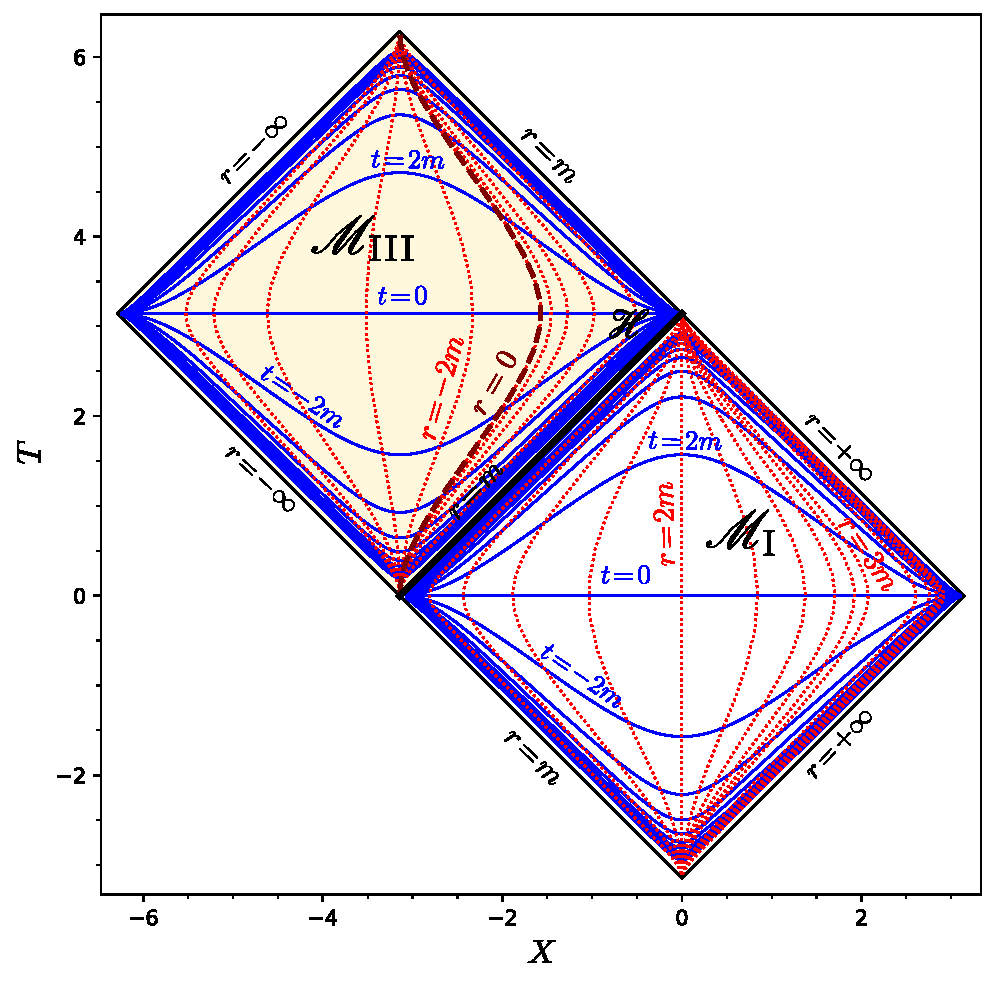
\includegraphics[width=0.8\textwidth]{exk_CPdiag_BL.pdf}}
\caption[]{\label{f:exk:CPdiag_BL} \footnotesize
Same as Fig.~\ref{f:exk:CPdiag_Kerr} but for the
time slicing associated to Boyer-Lindquist coordinates $(t,r,\th,\ph)$.
The blue curves represent hypersurfaces $t=\mathrm{const}$, with
$t\in[-20 m, 20 m]$ and
the increment $\delta t = 2 m$ between two successive hypersurfaces.
Note that the spacetime slicing by the hypersurfaces $t=\mathrm{const}$
is singular at $\Hor$, contrary to the slicing by the hypersurfaces
of constant Kerr time $\ti$ shown in Fig.~\ref{f:exk:CPdiag_Kerr}.
\textsl{[Figure generated by the notebook \ref{s:sam:Kerr_extremal}]}
}
\end{figure}

%%%%%%%%%%%%%%%%%%%%%%%%%%%%%%%%%%%%%%%%%%%%%%%%%%%%%%%%%%%%%%%%%%%%%%%%%%%%%%%

\section{Maximal analytic extension} \label{s:exk:max_extension}

\subsection{Extension of $\M_{\rm I}$ for complete outgoing principal null geodesics}

Figure~\ref{f:exk:CPdiag_Kerr} depicts a Carter-Penrose diagram of
the extremal Kerr spacetime $(\M,\w{g})$ built by means of the projection
map\footnote{cf. the definition of a Carter-Penrose diagram given in
Sec.~\ref{s:ker:Carter_Penrose_diag}.}
$\Pi: \M \to \R^2, (\ti, r, \th,\tph) \mapsto (T,X)$ defined by
\begin{subequations}
\label{e:exk:projection_M}
\begin{align}
   & T = T_0(u, v) \qand X = X_0(u, v) \quad\mbox{in}\ \M_{\rm I} \\
   & T = \arctan(v/2) + \pi/2 \qand X = \arctan(v/2) - \pi/2 \quad\mbox{on} \ \Hor \\
   & T = T_0(u, v) + \pi \qand X = X_0(u, v) - \pi \quad\mbox{in}\ \M_{\rm III}
\end{align}
\end{subequations}
with
\be \label{e:exk:def_T0_X0}
T_0(u, v) := \arctan\left(\frac{u}{2}\right) + \arctan\left(\frac{v}{2}\right) ,\qquad
X_0(u, v) := \arctan\left(\frac{v}{2}\right) - \arctan\left(\frac{u}{2}\right) ,
\ee
where $u$ and $v$ are the functions of $(\ti, r)$ given by
Eqs.~(\ref{e:exk:def_u}) and (\ref{e:exk:def_v}) respectively.
Some outgoing principal null geodesics
$\Li^{\rm out, I}_{(u,\th,\tilde{\tph})}$ and $\Li^{\rm out, III}_{(u,\th,\tilde{\tph})}$
are plotted in Fig.~\ref{f:exk:CPdiag_Kerr}
for selected values of $u$ (solid green lines): $u=-4m$, $u=0$ and $u=4m$.
Since $r$ is an affine parameter along the null geodesics $\Li^{\rm out, I}_{(u,\th,\tilde{\tph})}$,
it is clear that these geodesics are incomplete, for they all terminate
in the past at the finite value $r=m$ (the South-West boundary
of $\M_{\rm I}$ in Fig.~\ref{f:exk:CPdiag_Kerr}), without any possible
extension into $\M_{\rm III}$ from there.
To extend $\M_{\rm I}$ so that all geodesics $\Li^{\rm out, I}_{(u,\th,\tilde{\tph})}$
are complete, let us introduce a coordinate system on $\M_{\rm I}$ that is
adapted to the outgoing principal null geodesics, as the Kerr coordinates
$(\ti,r,\th,\tph)$ were adapted to the ingoing ones.
We thus define the \defin{outgoing Kerr coordinates}\index{outgoing!Kerr coordinates}\index{Kerr!coordinates!outgoing --} $(x^{\tilde{\tilde\alpha}})=(\tilde{\ti},r,\th,\tilde{\tph})$ by
\be \label{e:exk:ttt_u}
    u = \tilde{\ti} - r \iff \tilde{\ti} = u + r  ,
\ee
where $u$ is the retarded Kerr time (\ref{e:exk:def_u}) and $\tilde{\tph}$
is related to the angle $\tph$ of Kerr coordinates or to the angle
$\ph$ of Boyer-Lindquist coordinates by Eq.~(\ref{e:exk:def_ttph}).
Substituting Eq.~(\ref{e:exk:def_u}) for $u$ into $\tilde{\ti} = u + r$
and using Eq.~(\ref{e:exk:def_ttph}) linking $\tilde{\tph}$ to $\tph$,
we get the transition map between the Kerr coordinates $(\ti,r,\th,\tph)$
and the outgoing Kerr coordinates $(\tilde{\ti},r,\th,\tilde{\tph})$:
\be \label{e:exk:Kerr_to_out_Kerr}
    \mbox{on}\, \M_{\rm I},\quad  \left\{
    \begin{array}{l}
    \displaystyle \tilde{\ti}  = \ti + \frac{4 m^2}{r - m}
                        - 4 m \ln \left( \frac{r - m}{m} \right) \\[2ex]
    \displaystyle \tilde{\tph}  = \tph + \frac{2m}{r -m} .
    \end{array} \right.
\ee


By construction, the tangent vector to $\Li^{\rm out, I}_{(u,\th,\tilde{\tph})}$
associated with the affine parameter $r$ is then
\be \label{e:exk:def_ell_prime}
    \wl' = \wpar_{\tilde{\ti}} + \wpar_{\tilde{\tilde{r}}},
\ee
where $\wpar_{\tilde{\tilde{r}}}$ stands for the vector $\partial/\partial r$
of the coordinates $(\tilde{\ti},r,\th,\tilde{\tph})$.
Indeed ${\ell'}^{\tilde{\tilde\alpha}} = \D x^{\tilde{\tilde\alpha}} /\D r
= (1, 1, 0, 0)$ since along $\Li^{\rm out, I}_{(u,\th,\tilde{\tph})}$,
$\tilde{\ti} = r + u$, with $u$ constant, and both $\th$ and $\tilde{\tph}$
are constant. An explicit computation (cf. the notebook~\ref{s:sam:Kerr_extremal_extended}) shows that
$\wl'$ is a geodesic vector:
\be
    \wnab_{\wl'} \wl' = 0 ,
\ee
which confirms that $r$ is an affine parameter along $\Li^{\rm out, I}_{(u,\th,\tilde{\tph})}$.
$\wl'$ is thus similar to $\w{k}$, which is
the tangent vector to the \emph{ingoing} principal null geodesics $\Li^{\rm in}_{(v,\th,\tph)}$
associated with the affine parameter $-r$ along them.
In this respect, note the symmetry between the relations
$\wl' = \wpar_{\tilde{\ti}} + \wpar_{\tilde{\tilde{r}}}$
and $\w{k} = \wpar_{\ti} - \wpar_{\tilde{r}}$ [Eq.~(\ref{e:exk:k_3p1_Kerr})].
The link between $\wl'$ and the tangent vector $\wl$ to $\Li^{\rm out, I}_{(u,\th,\tilde{\tph})}$
introduced in Sec.~\ref{s:exk:princ_null_geod} is easily obtained from
the definition of a tangent vector to a curve:
\[
    \wl' = \frac{\D\w{x}}{\D r} = \frac{\D\w{x}}{\D\lambda} \frac{\D\lambda}{\D r}
        = \left(\frac{\D r}{\D \lambda} \right) ^{-1} \wl ,
\]
where $\lambda$ is the (non-affine) parameter of $\Li^{\rm out, I}_{(u,\th,\tilde{\tph})}$
associated with $\wl$. We read on the Kerr components (\ref{e:exk:ell_3p1_Kerr})
of $\wl$, as well as on the Boyer-Lindquist ones (\ref{e:exk:ell_BL}), that
$\D r/\D\lambda = \ell^r = (r-m)^2/(2(r^2 + m^2))$. Hence
\be \label{e:exk:ell_prime_ell}
    \wl' = 2 \frac{r^2 + m^2}{(r - m)^2} \, \wl .
\ee

Differentiating Eq.~(\ref{e:exk:Kerr_to_out_Kerr})
leads to
\be \label{e:exk:Dttt_Dtph_Kerr}
    \D\tilde{\ti} = \D\ti - \frac{4 m r}{(r-m)^2} \D r
    \qand
    \D\tilde{\tph} = \D\tph - \frac{2 m}{(r-m)^2} \D r .
\ee
From these relations and the chain rule, we get immediately
the link between the outgoing Kerr coordinate frame and the Kerr coordinate frame:
\be \label{e:exk:out_Kerr_frame}
    \wpar_{\tilde{\ti}} = \wpar_{\ti},\qquad
    \wpar_{\tilde{\tilde{r}}} = \wpar_{\tilde{r}} + \frac{4 m r}{(r-m)^2} \wpar_{\ti}
        + \frac{2m}{(r-m)^2} \wpar_{\tph}, \qquad
    \wpar_{\th} = \wpar_{\th},\qquad
    \wpar_{\tilde{\tph}} = \wpar_{\tph} .
\ee
In view of Eq.~(\ref{e:exk:Killing_vectors}), we conclude that
$\wpar_{\tilde{\ti}}$ and $\wpar_{\tilde{\tph}}$ coincide
with the Killing vectors $\w{\xi}$ and $\w{\eta}$ of the Kerr metric:
\be
    \wpar_{\tilde{\ti}} = \w{\xi} \qand \wpar_{\tilde{\tph}} = \w{\eta} .
\ee

The link between the outgoing Kerr coordinates and the Boyer-Lindquist ones
is obtained by substituting Eq.~(\ref{e:exk:def_u}) for $u$ into $\tilde{\ti} = u + r$
[Eq.~(\ref{e:exk:ttt_u})]:
\be \label{e:exk:ttt_t}
    \tilde{\ti} = t + \frac{2m^2}{r -m} - 2m\ln\left| \frac{r - m}{m} \right| .
\ee
This relation is to be supplemented by Eq.~(\ref{e:exk:def_ttph}) to fully
specify the transformation from the Boyer-Lindquist coordinates
$(t,r,\th,\ph)$ to the outgoing Kerr coordinates
$(\tilde{\ti},r,\th,\tilde{\tph})$.
Differentiating Eqs.~(\ref{e:exk:ttt_t}) and (\ref{e:exk:def_ttph})
leads to
\be \label{e:exk:Dttt_Dtph_BL}
    \dd\tilde{\ti} = \dd t - \frac{2 m r}{(r-m)^2} \dd r
    \qand
    \dd\tilde{\tph} = \dd\ph - \frac{m}{(r-m)^2} \dd r .
\ee
\begin{remark}
Equation~(\ref{e:exk:Dttt_Dtph_BL}) differs from
Eq.~(\ref{e:exk:dt_dph}) only by the sign $+$ changed to $-$ in the
right-hand side. This reflects the complete symmetry between the Kerr coordinates
$(\ti,r,\th,\tph)$
and the outgoing Kerr coordinates
$(\tilde{\ti},r,\th,\tilde{\tph})$
from the point of view of the Boyer-Lindquist coordinates $(t,r,\th,\ph)$
(cf. the discussion at the beginning of Sec.~\ref{s:ker:out_princ_null_geod}).
\end{remark}


The expression of the metric tensor with respect to the
outgoing Kerr coordinates is easily obtained by substituting $\dd t$ and $\dd\ph$
from Eq.~(\ref{e:exk:Dttt_Dtph_BL}) into the Boyer-Lindquist expression
(\ref{e:exk:metric_BL}) (see also the notebook~\ref{s:sam:Kerr_extremal_extended}); we get
\be \label{e:exk:metric_out_Kerr}
    \begin{array}{ll}
    \w{g}   = &
    \displaystyle - \left( 1 - \frac{2m r}{\rho^2} \right)  {\dd\tilde{\ti}}^2
    - \frac{4m r}{\rho^2} \dd\tilde{\ti}\, \dd r
    - \frac{4 m^2  r \sin^2\th}{\rho^2} \,  \dd\tilde{\ti}\, \dd\tilde{\tph}
      + \left( 1 + \frac{2m r}{\rho^2} \right) \dd r^2 \\[2ex]
    & \displaystyle + 2 m \left( 1 + \frac{2m r}{\rho^2} \right) \sin^2\th \, \dd r\, \dd\tilde{\tph} + \rho^2 \dd \th^2
    + \left( r^2 + m^2 + \frac{2 m^3 r \sin^2\th}{\rho^2} \right)
    \sin^2\th \, {\dd\tilde{\tph}}^2 .
    \end{array}
\ee
These metric components are very similar to those in Kerr coordinates, as given by
Eq.~(\ref{e:exk:metric_Kerr_3p1}): the only differences are $g_{\tilde{\ti}r}$ and
$g_{r\tilde{\tph}}$, which have a sign opposite to that of respectively $g_{\ti r}$
and $g_{r\tph}$. Apart from the standard singularities of the
spherical coordinates $(\th,\tilde{\tph})$ on the axis $\th\in\{0,\pi\}$, the
only singularity of the metric components (\ref{e:exk:metric_out_Kerr})
would occur at $\rho=0$, which does not happen in $\M_{\rm I}$. In particular
there is no divergence for $r\to m$. This can be used to extend smoothly
the spacetime $(\M_{\rm I},\w{g})$ to $r\in(-\infty, m]$, so that the outgoing
principal null geodesics $\Li^{\rm out, I}_{(u,\th,\tilde{\tph})}$
with $\th\neq \pi/2$ become
complete. But the extension to $r<m$ cannot be $\M_{\rm III}$
as it appears clearly on Fig.~\ref{f:exk:CPdiag_Kerr} that  the end point
of $\Li^{\rm out, I}_{(u,\th,\tilde{\tph})}$ for $r\to m^+$ is not located at the
boundary between $\M_{\rm I}$ and $\M_{\rm III}$.
We thus introduce a spacetime $(\M',\w{g})$ from a new copy of
$\R^2\times\SS^2$ with $\R^2$ spanned by the coordinates $(\tilde{\ti},r)$ and
$\SS^2$ spanned by the coordinates $(\th,\tilde{\tph})$, such that (i)
the manifold $\M'$ is
\be
 \M' := \R^2\times\SS^2 \setminus \ring'
 \quad\mbox{where}\quad
    \ring' := \left\{ p \in \R^2\times\SS^2,
        \quad r(p) = 0 \ \mbox{and}\ \th(p) = \frac{\pi}{2} \right\} ,
\ee
(ii) $\M_{\rm I}$ is identified with the part $r>m$ of $\M'$ and
(iii) in all $\M'$, $\w{g}$ has the components given by expression
(\ref{e:exk:metric_out_Kerr}). Furthermore, we define
\be
    \Hor' := \left\{ p \in \M', \quad r(p) = m \right\}
    \qand
    {\M'}_{\rm III} := \left\{ p \in \M', \quad r(p) < m \right\} .
\ee
We have then $\M_{\rm I} = \M \cap \M'$.
In ${\M'}_{\rm III}$, one can define Kerr coordinates $(\ti,r,\th,\tph)$
from $(\tilde{\ti},r,\ph,\tilde{\tph})$
via formulas (\ref{e:exk:def_u}) (with $u = \tilde{\ti} - r$) and (\ref{e:exk:def_ttph}).
It appears then immediately that $({\M'}_{\rm III}, \w{g})$ is isometric to $(\M_{\rm III},\w{g})$.
It follows that $\w{g}$ obeys the vacuum Einstein equation in all $\M'$.
The vector field $\wl' := \wpar_{\tilde{\ti}} + \wpar_{\tilde{\tilde{r}}}$
[cf. Eq.~(\ref{e:exk:def_ell_prime})] is a smooth non-vanishing null vector
field on $\M'$. Since it is future directed in $(\M_{\rm I},\w{g})$
considered as a part of $(\M,\w{g})$,
we use it to set the time orientation in all $\M'$.

The tangent vector $\w{k}$ to ingoing principal null geodesics has
the following components with respect to the outgoing Kerr coordinates:
\be \label{e:exk:k_out_Kerr}
    \w{k} = \frac{(r + m)^2}{(r - m)^2} \, \wpar_{\tilde{\ti}}
    - \wpar_{\tilde{\tilde{r}}} + \frac{2m}{(r - m)^2} \, \wpar_{\tilde{\tph}} .
\ee
This follows immediately from
$\w{k} = \wpar_{\ti} - \wpar_{\tilde{r}}$ [Eq.~(\ref{e:exk:k_3p1_Kerr})]
and using Eq.~(\ref{e:exk:out_Kerr_frame})
to substitute $\wpar_{\ti}$ and $\wpar_{\tilde{r}}$.
Extending Equation~(\ref{e:exk:k_out_Kerr}) to all $\M'$
leads to a vector field that is singular on $\Hor'$. To get a vector field
everywhere regular on $\M'$, we rescale it by the inverse of the factor
connecting $\wl$ to $\wl'$ in Eq.~(\ref{e:exk:ell_prime_ell}), i.e. we
define
\be
    \w{k}' := \frac{(r - m)^2}{2(r^2 + m^2)} \, \w{k} .
\ee
Hence
\be \label{e:exk:k_prime_out_Kerr}
    \w{k}' = \frac{(r + m)^2}{2(r^2 + m^2)} \, \wpar_{\tilde{\ti}}
    - \frac{(r-m)^2}{2(r^2 + m^2)}\, \wpar_{\tilde{\tilde{r}}} + \frac{m}{r^2 + m^2} \, \wpar_{\tilde{\tph}} .
\ee
This vector field is clearly regular in all $\M'$.
Accordingly, it can be used to extend smoothly the family of ingoing principal
null geodesics to $\Hor'$. The price to pay is that $\w{k}'$ is only a pregeodesic
vector field, while $\w{k}$ was geodesic, being associated with the affine parameter $-r$.
The pair $(\w{k}, \w{k}')$ plays actually the same role as the pair $(\wl', \wl)$
(note the order!) regarding the outgoing principal null geodesics.

\begin{figure}
\centerline{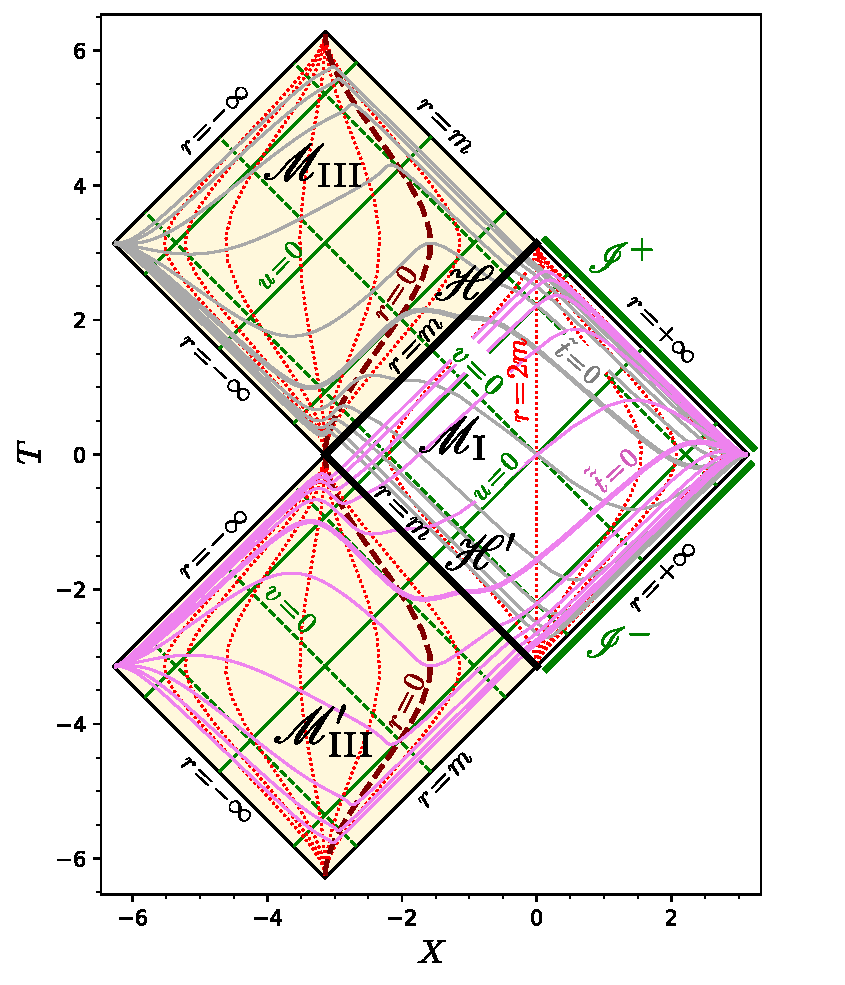
\includegraphics[width=0.8\textwidth]{exk_CPdiag_M0.pdf}}
\caption[]{\label{f:exk:CPdiag_M0} \footnotesize
Carter-Penrose diagram of the (partially) extended extremal Kerr spacetime $(\M_0,\w{g})$.
The grey curves represent hypersurfaces $\ti=\mathrm{const}$ in $\M$, with
$\ti\in[-10 m, 10 m]$ and
the increment $\delta\ti = 2 m$ between two successive hypersurfaces.
The hypersurface $\ti=0$ is singled out by a larger thickness.
The purple curves represent hypersurfaces $\tilde{\ti}=\mathrm{const}$ in $\M'$, with
$\tilde{\ti}\in[-10 m, 10 m]$ and
the increment $\delta\tilde{\ti} = 2 m$ between two successive hypersurfaces.
The hypersurface $\tilde{\ti}=0$ is singled out by a larger thickness.
The red dotted curves represent hypersurfaces $r=\mathrm{const}$,
with the increment $\delta r$ between two successive hypersurfaces being
$\delta r = 2m$ for $r<0$ and $r> 3m$ and $\delta r = 0.5\, m$ for $0\leq r \leq 3m$.
The hypersurfaces $r=0$ are marked by brown dashed curves.
The dashed (resp. solid) green straight lines depict some selected ingoing (resp. outgoing)
principal null geodesics.
\textsl{[Figure generated by the notebook \ref{s:sam:Kerr_extremal_extended}]}
}
\end{figure}

As $\Hor$ in $(\M,\w{g})$, $\Hor'$ is a degenerate Killing horizon of $(\M',\w{g})$.
Indeed, by the same reasoning as in Sec.~\ref{s:exk:horizon}, we get that
the null normal to $\Hor'$ is the Killing vector
$\w{\chi} = \w{\xi} + 1/(2m) \, \w{\eta}$ [Eq.~(\ref{e:exk:def_chi}) extended to
$\M'$]. This normal coincides with $\w{k}'$ on $\Hor'$, as we can see
by setting $r=m$ in  Eq.~(\ref{e:exk:k_prime_out_Kerr}). This implies that
the null geodesic generators of  $\Hor'$ belong to the ingoing principal null congruence.
The non-affinity coefficient of $\w{k}'$ is (cf. the notebook~\ref{s:sam:Kerr_extremal_extended}):
\be
    \kappa_{\w{k}'} = m \frac{m^2 - r^2}{(r^2 + m^2)^2} .
\ee
We have thus $\kappa_{\w{k}'} = 0$ on $\Hor'$, so that $\Hor'$ is a
degenerate Killing horizon.

With $\M'$, our extended extremal Kerr spacetime is thus $(\M_0,\w{g})$ with
\be
   \encadre{ \M_0 := \M \cup \M'
     = \M_{\rm I} \cup \M_{\rm III} \cup \M'_{\rm III} \cup \Hor \cup \Hor' } .
\ee
A Carter-Penrose diagram of $\M_0$ is shown in Fig.~\ref{f:exk:CPdiag_M0}.
The projection operator used to build this diagram (cf. Sec.~\ref{s:ker:Carter_Penrose_diag})
is $\Pi : \M_0 \to \R^2$, with $\R^2$ spanned by coordinates $(T,X)$,
such that $\Pi$ is defined by Eqs.~(\ref{e:exk:projection_M})-(\ref{e:exk:def_T0_X0})
on $\M$, while on $\M'$, $\Pi$ is defined by
\begin{subequations}
\begin{align}
   & T = T_0(u, v) \qand X = X_0(u, v) \quad\mbox{in}\ \M_{\rm I} \\
   & T = \arctan(u/2) - \pi/2 \qand X = -\arctan(u/2) - \pi/2 \quad\mbox{on} \ \Hor' \\
   & T = T_0(u, v) - \pi \qand X = X_0(u, v) - \pi \quad\mbox{in}\ \M'_{\rm III}
\end{align}
\end{subequations}
where $T_0(u,v)$ and $X_0(u,v)$ are given by Eq.~(\ref{e:exk:def_T0_X0})
and $u$ and $v$ are functions of $(\tilde{\ti}, r)$ defined by
respectively $u = \tilde{\ti} - r$ [Eq.~(\ref{e:exk:ttt_u})]
and
\be
    v = \tilde{\ti} + r - \frac{4 m^2}{r - m} + 4 m \ln \left| \frac{r - m}{m} \right| .
\ee
The last equation is obtained by combining Eqs.~(\ref{e:exk:def_v}) and (\ref{e:exk:def_u}).


\begin{remark}
As we have constructed it, the manifold $\M_0$ is covered by two coordinate charts:
$(\ti, r, \th, \tph)$ on $\M_{\rm I} \cup \Hor \cup \M_{\rm III}$
and $(\tilde{\ti}, r, \th, \tilde{\tph})$ on $\M_{\rm I} \cup \Hor' \cup \M'_{\rm III}$.
These two charts overlap in $\M_{\rm I}$, where the transition between them
is provided by Eq.~(\ref{e:exk:Kerr_to_out_Kerr}).
The Carter-Penrose diagram of Fig.~\ref{f:exk:CPdiag_M0} might give the impression
that, by means of the coordinates $(T,X)$, one could cover $\M_0$ by a single chart,
in a fashion similar to the covering of the entire maximal extension of Schwarzschild
spacetime by the Kruskal-Szekeres coordinates\index{Kruskal-Szekeres!coordinates}
$(T,X,\th,\ph)$ (cf. Sec.~\ref{s:sch:max_extens}). However, this is not possible
in a simple way, due to singularity issues with the azimuthal coordinates:
$\tph$ diverges on $\Hor'$, $\tilde{\tph}$ diverges on $\Hor$ and
the Boyer-Lindquist coordinate $\ph$ diverges on both $\Hor$ and $\Hor'$.
Accordingly, none of $(T,X,\th,\tph)$, $(T,X,\th,\tilde{\tph})$ and
$(T,X,\th,\ph)$ would provide a regular chart of $\M_0$.
\end{remark}

\begin{remark} \label{r:exk:M0_analytic}
The spacetime $(\M_0,\w{g})$ is analytic: (i) $\M_0$ is an analytic manifold,
given that the change of coordinates (\ref{e:exk:Kerr_to_out_Kerr})
between the two charts covering $\M_0$ is analytic
(cf. Remark~\ref{r:bas:analytic} in Sec.~\ref{s:bas:def_manif})
and (ii) the components (\ref{e:exk:metric_Kerr_3p1}) and (\ref{e:exk:metric_out_Kerr})
of $\w{g}$ are analytic functions of the
coordinates $(\ti, r, \th, \tph)$ and $(\tilde{\ti}, r, \th, \tilde{\tph})$
respectively.
\end{remark}


The Killing horizon $\Hor'$ is actually a white hole horizon from the point
of view of $\M_{\rm I}$. More precisely, we can endow $(\M_0,\w{g})$ with the same conformal
completion at null infinity as that used for $(\M,\w{g})$ in Sec.~\ref{s:exk:bhole_char},
i.e. such that the conformal boundary $\scri$ is constituted by
the same future and past null infinities
$\scri^+$ and $\scri^-$ located at the boundary of $\M_{\rm I}$ (cf. Fig.~\ref{f:exk:CPdiag_M0}).
It appears then that
\be
   \M'_{\rm III}\cup \Hor' = \M_0 \setminus (J^+(\scri^-)\cap \M_0)
\ee
In view of the definition (\ref{e:glo:def_white_hole}), we conclude:
\begin{prop}[white hole region in the extended extremal Kerr spacetime]
$\M'_{\rm III}$ is the interior of a white hole\index{white hole} region, the boundary of which
is $\Hor'$.
\end{prop}

Since $\M_{\rm III}$ was shown in Sec.~\ref{s:exk:bhole_char} to be the black hole region for
the same conformal completion at null infinity, we may state,
according to the terminology introduced in Sec.~\ref{s:glo:def_BH}:
\begin{prop}[domain of outer communications]
$\M_{\rm I}$ is the domain of outer communications\index{domain of outer communications}
of the spacetime $(\M_0,\w{g})$.
\end{prop}


\begin{figure}
\centerline{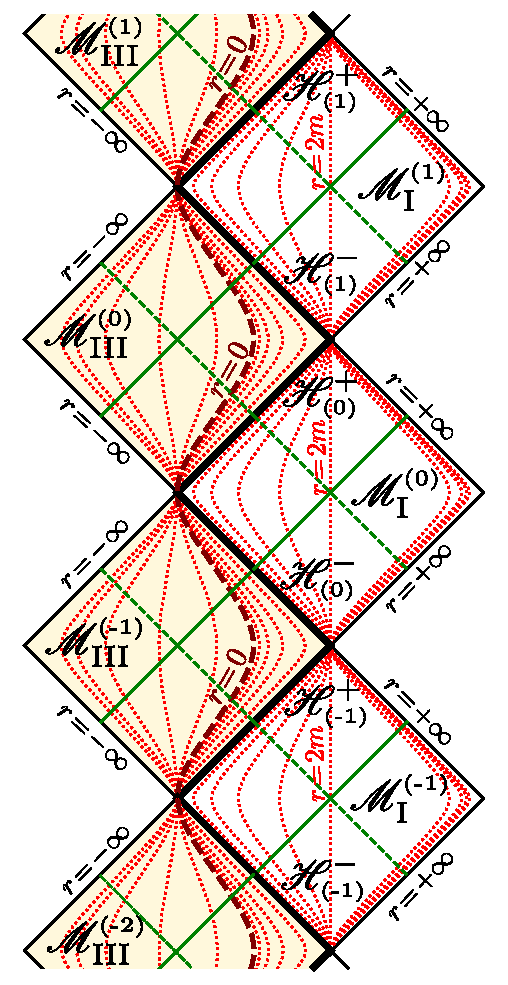
\includegraphics[height=0.7\textheight]{exk_CPdiag_maximal.pdf}}
\caption[]{\label{f:exk:CPdiag_maximal} \footnotesize
Carter-Penrose diagram of the maximal analytic extension $(\M_*,\w{g})$
of the extremal Kerr spacetime.
The red dotted curves represent hypersurfaces $r=\mathrm{const}$,
with the increment $\delta r$ between two successive hypersurfaces being
$\delta r = 2m$ for $r<0$ and $r> 2m$ and $\delta r = 0.2\, m$ for $0\leq r \leq 2m$.
The hypersurfaces $r=0$ are marked by brown dashed curves.
The dashed (resp. solid) green straight lines depict ingoing (resp. outgoing)
principal null geodesics with $v=0$ (resp. $u=0$).
\textsl{[Figure generated by the notebook \ref{s:sam:Kerr_extremal_extended}]}
}
\end{figure}

\subsection{Construction of the maximal analytic extension}

With $(\M_0,\w{g})$, we have achieved our first goal: all the outgoing
principal null geodesics crossing $\M_{\rm I}$ and not lying in the equatorial
plane (i.e. the geodesics extending the $\Li^{\rm out, I}_{(u,\th,\tilde{\tph})}$
family with $\th\neq \pi/2$ to the past) are complete. However, there remains
incomplete geodesics in $\M_0$: the outgoing principal null geodesics crossing $\M_{\rm III}$
all stop at the value $r=m$ of their affine parameter, while
the ingoing principal null geodesics crossing $\M'_{\rm III}$ all start at the
value $-r = -m$ of their affine parameter (cf. Fig.~\ref{f:exk:CPdiag_M0}).
To construct a spacetime with complete geodesics, except for those that encouter the curvature singularity at $r=0$ and $\th=\pi/2$, one introduces an infinite number of copies of $\M_0$,
$\left( \M_n \right)_{n\in\mathbb{Z}}$ say, and identify the region $\M'_{\rm III}$ of $\M_n$
with the region $\M_{\rm III}$ of $\M_{n-1}$ for all $n\in\mathbb{Z}$.
The manifold hence obtained,
\be
    \M_* := \bigcup_{n\in\mathbb{Z}} \M_n ,
\ee
is depicted via a
Carter-Penrose diagram in Fig.~\ref{f:exk:CPdiag_maximal}.
The region $\M_{\rm I}$ (resp. $\M_{\rm III}$) of $\M_n$ is
denoted by $\M_{\rm I}^{(n)}$ (resp. $\M_{\rm III}^{(n)}$). Similarly,
the Killing horizon $\Hor$ (resp. $\Hor'$) of $\M_n$ is denoted
by $\Hor_{(n)}^+$ (resp. $\Hor_{(n)}^-$). Note that $\Hor_{(n)}^+$
is a future event horizon (black hole horizon), while
$\Hor_{(n)}^-$ is a past event horizon (white hole horizon),
for the conformal completion at null infinity with
the future and past null infinities $\scri^+_{(n)}$ and $\scri^-_{(n)}$
as copies of $\scri^+$ and $\scri^-$ introduced for $\M_0$.

It is clear that $(\M_*,\w{g})$ is an analytic spacetime, since $(\M_0,\w{g})$
is (cf. Remark~\ref{r:exk:M0_analytic} on p.~\pageref{r:exk:M0_analytic}).

By construction, all principal null geodesics are complete in $\M_*$,
except for those that encounter the curvature singularity at
$r=0$ and $\th=\pi/2$. In particular, this holds for the outgoing
principal null geodesics generating $\Hor_{(n)}^+$
and for the ingoing ones generating $\Hor_{(n)}^-$.
Contemplating the Carter-Penrose diagram of Fig.~\ref{f:exk:CPdiag_maximal},
we might thus perceive each (solid or dashed) green straight line
from an $r=-\infty$ end to an $r=+\infty$ end, as well as
each thick black straight line, as representing a complete principal null
geodesic.

It can be shown that actually \emph{all} timelike or null
geodesics of $(\M_*,\w{g})$, and not only the principal null ones, are complete
(see Carter's article \cite{Carte68a} for the proof), so that we can conclude:
\begin{prop}[maximal analytic extension of the extremal Kerr spacetime]
$(\M_*,\w{g})$ is the maximal analytic extension of the
extremal Kerr spacetime.
\end{prop}

\begin{remark}
The construction of the maximal extension of the extremal Kerr spacetime
is simpler than that of the Kerr spacetime with $a<m$ presented
in Sec.~\ref{s:ker:max_extension}. Indeed, for the latter, if one uses
only the ingoing and outgoing Kerr coordinate patches $(\ti,r,\th,\tph)$
and $(\tilde{\ti},r,\th,\tilde{\tph})$, one ends up with a manifold that
is not maximal: the null geodesics generating the Killing horizons
at $r=r_\pm$ are not complete, because the bifurcation spheres\index{bifurcation!sphere}
(the central dots in Fig.~\ref{f:ker:max_ext}), accross which these geodesics
can be extended, are missing.
Indeed the bifurcation spheres are not covered by Kerr coordinates.
To include them and thus get the full bifurcate Killing horizons
(cf. Sec.~\ref{s:sta:bifur_Killing_hor}), one has to introduce Kruskal-Szekeres-type
coordinates in the vicinity of each bifurcation sphere, in a way similar to
the Schwarzschild case treated in Secs.~\ref{s:max:KS} and \ref{s:sch:max_extens}.
In the present case, each Killing horizon $\Hor^+_{(n)}$ or $\Hor^-_{(n)}$
is degenerate and therefore made of complete null geodesics. In particular,
$\Hor^+_{(n)}$ and $\Hor^-_{(n)}$ are not part of a bifurcate Killing horizon. In other words, there
is no bifurcation sphere in the maximal extension of the extremal Kerr spacetime
and the ingoing and outgoing Kerr coordinate patches
are sufficient to cover it entirely.
\end{remark}

\begin{hist}
In 1966, Brandon Carter\index[pers]{Carter, B.} \cite{Carte66} obtained the maximal analytic extension
of the rotation axis $\mathscr{A}$ of the extremal Kerr spacetime (cf. historical note on p.~\pageref{h:ker:max_ext_diag}). In particular, he drew a diagram (Fig.~1b of Ref.~\cite{Carte66})
similar to that of Fig.~\ref{f:exk:CPdiag_maximal}, the difference
being that Carter's one is a true conformal representation, owing to the fact
that $\mathscr{A}$ is 2-dimensional, while the diagram of Fig.~\ref{f:exk:CPdiag_maximal}
is a mere projection of the 4-dimensional manifold $\M_*$.
In their 1967 classical study entitled \emph{Maximal Analytic Extension of the Kerr metric}
\cite{BoyerL67},
Robert H. Boyer\index[pers]{Boyer, R.H.} and Richard W. Lindquist\index[pers]{Lindquist, R.W.}
focused on the case $a<m$. For $a=m$, they referred to Carter's study \cite{Carte66}
and stated simply that
\emph{although his
\emph{[Carter's]} work was confined to the symmetry axis ($\th=0,\pi$), it is clear
that his conclusions apply with equal force to the full metric}.
The detailed construction of the maximal analytic extension
of the full extremal Kerr spacetime was actually presented by Carter himself
in 1968 \cite{Carte68a}, as the special case of vanishing electric charge
of the extremal Kerr-Newman spacetime.
The construction was also performed in details in his famous lectures at Les Houches
Summer School in 1972~\cite{Carte73a}.
\end{hist}


%%%%%%%%%%%%%%%%%%%%%%%%%%%%%%%%%%%%%%%%%%%%%%%%%%%%%%%%%%%%%%%%%%%%%%%%%%%%%%%

\section{Near-horizon extremal Kerr (NHEK) geometry} \label{s:exk:NHEK}

\subsection{The extremal Kerr throat} \label{s:exk:throat}

Let us consider a hypersurface $\Sigma_t$ of constant Boyer-Lindquist time $t$
in the external region $\M_{\rm I}$ of the extremal Kerr spacetime, i.e.
one of the hypersurfaces shown in blue in Figs.~\ref{f:exk:BL_slicing}
and \ref{f:exk:CPdiag_BL}.
$\Sigma_t$ is a spacelike hypersurface, since it is clear from
the line element (\ref{e:exk:metric_BL}) that the metric induced by $\w{g}$
on $\Sigma_t$ is Riemannian (i.e. positive definite) in\footnote{The induced
metric would not be Riemannian in the Carter time machine (cf. Sec.~\ref{s:ker:time_machine}),
where $g_{\ph\ph} < 0$;
but this requires $r<0$, while $r>m$ in $\M_{\rm I}$.}
$\M_{\rm I}$.
We may thus visualize the geometry of $\Sigma_t$ by some isometric embedding
of 2-dimensional slices of $\Sigma_t$ into the Euclidean space $\R^3$,
as we did in Sec.~\ref{s:max:isometric_emb}
for the hypersurfaces of constant Kruskal-Szekeres time in
Schwarzschild spacetime. It is then
natural to consider the slices $\Sigma_{t,\th}$ where $\th$ is held constant,
in addition to $t$, with $\Sigma_{t,\frac{\pi}{2}}$ representing the
equatorial ``plane''. $\Sigma_{t,\th}$  is spanned by the coordinates
$(x^a) = (r,\ph)$ and the Riemannian metric $\w{q}$ induced on it by
the spacetime metric $\w{g}$ is obtained by setting $\dd t = 0$ and $\dd\th = 0$
in (\ref{e:exk:metric_BL}):
\be \label{e:exk:induced_metric_q}
    \w{q} =
    \frac{r^2 + m^2\cos^2\th}{(r-m)^2} \, \dd r^2
    + \left( r^2 + m^2 + \frac{2 m^3 r \sin^2\th}{r^2 + m^2\cos^2\th} \right)
    \sin^2\th \, \dd \ph^2 .
\ee
On the other side, the Euclidean space $\R^3$ can be described by
cylindrical coordinates $(X^i) = (\varpi,z,\ph)$, such that the
Euclidean metric $\w{f}$ takes the form
\be
    \w{f} = \dd \varpi^2 + \dd z^2 + \varpi^2 \dd\ph^2 .
\ee
Let us define the embedding of the 2-surface $\Sigma_{t,\th}$ into
$\R^3$ by
\be \label{e:exk:def_isom_emb}
    \begin{array}{clcl}
    \Phi: & \Sigma_{t,\th} & \longrightarrow & \R^3 \\
        & (r,\ph) & \longmapsto & (\varpi(r),z(r),\ph) .
    \end{array}
\ee
Along $\Phi(\Sigma_{t,\th})$, we have then
$\dd\varpi = \varpi'(r) \, \dd r$ and $\dd z = z'(r) \, \dd r$, so that the
metric $\w{h}$ induced by $\w{f}$ on $\Phi(\Sigma_{t,\th})$ is
\be \label{e:exk:induced_metric_h}
    \w{h} =
    \left( \varpi'(r)^2 + z'(r)^2 \right) \, \dd r^2
    + \varpi(r)^2 \, \dd\ph^2 .
\ee
$\Phi$ performs an isometric embedding iff the two metrics
(\ref{e:exk:induced_metric_q}) and (\ref{e:exk:induced_metric_h})
coincide\footnote{Formally, one says that the metric $\w{q}$ is the pullback
of $\w{h}$ by $\Phi$: $\w{q} = \Phi^* \w{h}$.}, i.e. iff
\begin{subequations}
\begin{align}
    & \varpi(r) = \sin\th \sqrt{r^2 + m^2 + \frac{2 m^3 r \sin^2\th}{r^2 + m^2\cos^2\th} }
        \label{e:exk:isom_emb_cond1} \\
    &\varpi'(r)^2 + z'(r)^2 = \frac{r^2 + m^2\cos^2\th}{(r-m)^2}  . \label{e:exk:isom_emb_cond2}
\end{align}
\end{subequations}
We deduced from Eq.~(\ref{e:exk:isom_emb_cond2}) that
\be \label{e:exk:isom_emb_z_r}
    z(r) = \int_{2m}^r
    \frac{1}{\bar{r}-m}
    \sqrt{\bar{r}^2 + m^2\cos^2\th
        - \varpi'(\bar{r})^2 (\bar{r}-m)^2 } \; \D \bar{r} ,
\ee
up to some additive constant, which we set to zero by choosing arbitrarily $z(2m) = 0$.
In the integrand, $\varpi'(\bar{r})$ should be substituted by the value obtained
by differentiating Eq.~(\ref{e:exk:isom_emb_cond1}).

\begin{figure}
\centerline{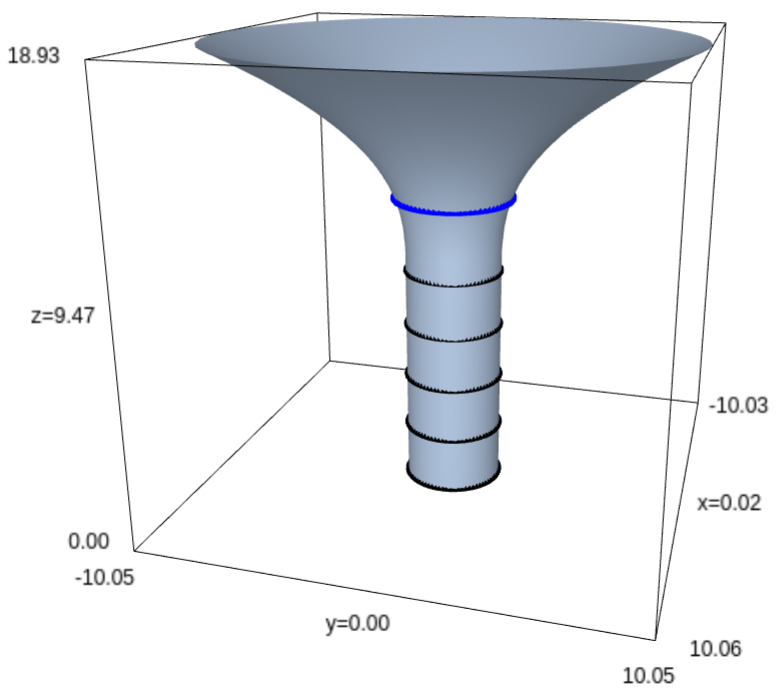
\includegraphics[width=0.6\textwidth]{exk_throat_emb_equat.png}
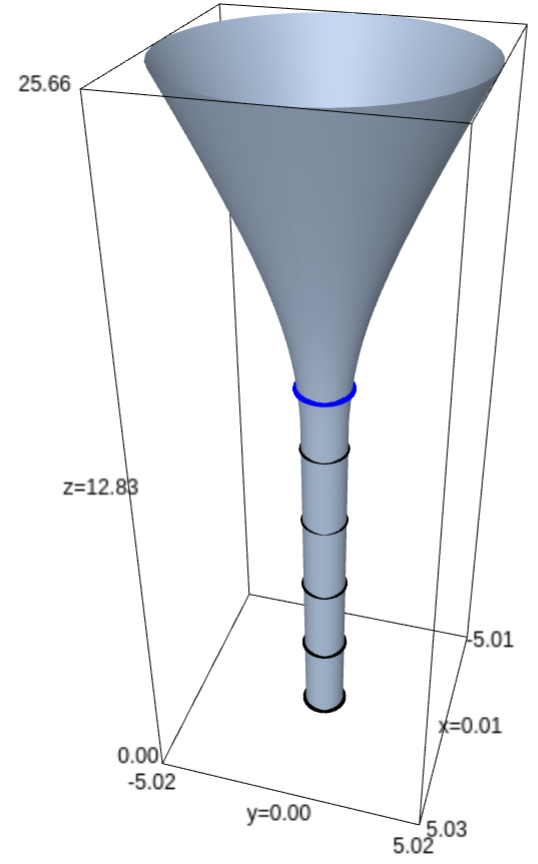
\includegraphics[width=0.35\textwidth]{exk_throat_emb_pi6.png}
}
\caption[]{\label{f:exk:throat_emb} \footnotesize
Isometric embeddings of 2-surfaces $\Sigma_{t,\th}$ of constant Boyer-Lindquist time $t$
and constant $\th$ of the extremal Kerr spacetime in the Euclidean 3-space,
for two values of $\th$: $\th=\pi/2$ (equatorial plane) (left figure)
and $\th=\pi/6$ (right figure). The drawings are truncated at
$r=(1 + 10^{-5})m$ (bottom boundary) and at $r=10\, m$
(top boundary). The blue circle marks the ergosphere, which is located at
$r=2m$ for $\th=\pi/2$ and $r=3m/2$ for $\th=\pi/6$. The five black circles
correspond to $r = 1.1\, m$, $1.01\, m$, $1.001\, m$, $1.0001\, m$
and $1.00001\, m$, from top to bottom.
\textsl{[Figure generated by the notebook \ref{s:sam:Kerr_extremal_throat_emb}]}
}
\end{figure}

The functions $\varpi(r)$ and $z(r)$, provided respectively by Eqs.~(\ref{e:exk:isom_emb_cond1})
and (\ref{e:exk:isom_emb_z_r}), define fully the isometric embedding
(\ref{e:exk:def_isom_emb}) of the Riemannian 2-manifold $(\Sigma_{t,\th}, \w{q})$ into
the Euclidean space $(\R^3,\w{f})$.
The outcome is depicted in Fig.~\ref{f:exk:throat_emb}
for two values of $\th$: $\pi/2$ (left plot) and $\pi/6$ (right plot).
In both cases, it appears that the embedded surface is infinite in two limits:
for $r\to +\infty$ and for $r\to m$.

The first limit, which implies $\varpi \to +\infty$ and $z \to +\infty$
according to Eqs.~(\ref{e:exk:isom_emb_cond1}) and (\ref{e:exk:isom_emb_z_r}),
is towards the asymptotic flat end of $\M_{\rm I}$.
More precisely, since $t$ is held fixed on $\Sigma_{t,\th}$, the asymptotic
direction appears as the
spacelike infinity\index{spacelike!infinity} point $i^0$ at the right-most corner
of the Carter-Penrose diagram of Fig.~\ref{f:exk:CPdiag_BL}.

The second limit, $r\to m$, corresponds to
$\varpi \to 2m\frac{\sin\th}{\sqrt{1 + \cos^2\th}}$ and $z\to -\infty$,
according to Eqs.~(\ref{e:exk:isom_emb_cond1}) and (\ref{e:exk:isom_emb_z_r}).
This describes an infinite cylinder, since
$\varpi$ tends to a constant value, while $z$ decays to $-\infty$.
The divergence of $z$ for $r\to m$ is of course due to the
factor $(\bar{r} - m)^{-1}$ in the integrand of (\ref{e:exk:isom_emb_z_r}),
which leads to the following behavior:
\be
    z(r) \sim m \sqrt{1 + \cos^2\th} \, \ln \left( \frac{r - m}{m} \right)
    \quad\mbox{when}\quad r\to m .
\ee
This logarithmic divergence is clearly apparent in Fig.~\ref{f:exk:throat_emb}:
the circles at $r - m = 10^{-1} m$, $10^{-2} m$, ..., $10^{-5} m$ look
equally spaced, all the more than $r$ is close to $m$.
In the Carter-Penrose diagram of Fig.~\ref{f:exk:CPdiag_BL}, the limit $r\to m$
at fixed $t$ appears as the point marked $i^{\rm int}$. This point is actually
the projection of a 2-sphere (spanned by $(\th,\ph)$) called
the \defin{internal infinity of the extremal Kerr spacetime}\index{internal!infinity}\index{infinity!internal --}. Let us stress that, as the spacelike infinity $i^0$
and the null infinities $\scri^+$ and $\scri^-$, the sphere $i^{\rm int}$
is not part of the physical spacetime $(\M,\w{g})$.

The property of $i^{\rm int}$ being located infinitely far from any point at $r=r_0>m$ on
a hypersurface $\Sigma_t$ appears clearly
on the metric (\ref{e:exk:metric_BL}). Indeed,
according to the latter, the distance along a
curve $(t,\th,\ph)=\mathrm{const}$ between the points
at $r=r_0$ and $r=m$ is
\[
    \ell = \int_{m}^{r_0} \sqrt{g_{rr}} \, \D r =
    \int_{m}^{r_0} \frac{\sqrt{r^2 + m^2\cos^2\th}}{r - m} \, \D r .
\]
Again, the factor $(r - m)^{-1}$ makes the integral diverge, so that $\ell = +\infty$.

Another perspective of $i^{\rm int}$ being ``infinitely far'' is obtained by noticing
that on the Carter-Penrose diagram of Fig.~\ref{f:exk:CPdiag_BL},
$i^{\rm int}$ is located at the past end of the event horizon $\Hor$. Since
$\Hor$ is a degenerate Killing horizon (cf. Sec.~\ref{s:exk:horizon}), it is generated by
\emph{complete} null geodesics: the principal null geodesics $\Li^{{\rm out},\Hor}_{(\th,\psi)}$
introduced in Sec.~\ref{s:exk:princ_null_geod}. Now, since
$\Li^{{\rm out},\Hor}_{(\th,\psi)}$ is complete, its past end at $i^{\rm int}$ is obtained at the limit $\ti\to -\infty$ of its
affine parameter $\ti$ (see also the grey curves in Fig.~\ref{f:exk:CPdiag_Kerr}, which let appear that
the limit $\ti\to -\infty$ at $r=m$ is
$i^{\rm int}$). Hence, in terms of affine length, $i^{\rm int}$ is infinitely
far in the past along any of the null geodesics $\Li^{{\rm out},\Hor}_{(\th,\psi)}$
generating $\Hor$.

The spacetime region in the vicinity of $r=m$ is called the
\defin{extremal Kerr throat}\index{extremal!Kerr!throat}\index{throat!extremal Kerr --}.
We are going to explore it in more details in the next sections.

\subsection{The NHEK metric} \label{s:exk:NHEK_metric}

In order to zoom in on the near-horizon region, let us introduce
a small parameter $\veps >0$ and
the \defin{Bardeen-Horowitz coordinates}\index{Bardeen-Horowitz coordinates}\footnote{Cf. the historical note on
page~\pageref{h:exk:NHEK_metric}.} $(T,R,\th,\Phi)$, which are defined on $\M_{\rm BL} = \M_{\rm I} \cup \M_{\rm III}$
and related to the Boyer-Lindquist coordinates
$(t,r,\th,\ph)$ by
\be \label{e:exk:def_R_T_Phi}
    t = 2m \frac{T}{\veps},\quad
    r = m (1 + \veps R),\quad
    \ph = \Phi + \frac{T}{\veps} ,
\ee
the reverse transformation being
\be \label{e:exk:R_T_Phi_BL}
    T = \veps \frac{t}{2m}, \quad
    R = \frac{r - m}{\veps m}, \quad
    \Phi = \ph - \frac{t}{2m} .
\ee
Note that on $\M_{\rm BL}$, the range of $T$ is $\R$, while
that of $R$ is $(-\infty,0)\cup(0,+\infty)$, with $R>0$ on $\M_{\rm I}$
and $R<0$ on $\M_{\rm III}$.
The coordinate choice (\ref{e:exk:def_R_T_Phi}) ensures, for a fixed value of $(T,R,\Phi)$ with $T>0$,
\be
    \lim_{\veps\to 0} t = +\infty,\quad
    \lim_{\veps\to 0} r = m, \quad
    \lim_{\veps\to 0} \ph = +\infty,\quad
    \frac{\D\ph}{\D t} = \frac{1}{2m}
\ee
and is motivated as follows.
For $\veps\to 0$,
the coordinate $R$ clearly implements the zoom on the region $r\simeq m$,
i.e. the region close to the event horizon $\Hor$.
Regarding the change $t\to T$, we may notice that the Boyer-Lindquist coordinate
$t$ diverges near  $\Hor$ --- more precisely,
$t$ diverges along the worldline of any particle that reaches $\Hor$
(this is clear on Figs.~\ref{f:exk:BL_slicing} and \ref{f:exk:CPdiag_BL}).
So, we may keep $T = \veps t/(2m)$ finite in the vicinity of $\Hor$, while having
$t$ diverging. The division by $2m$ makes $T$ dimensionless, as $R$, with the
factor $2$ being chosen for further convenience.
Similarly, the Boyer-Lindquist coordinate $\ph$ diverges along the worldline of any particle that reaches $\Hor$.
For geodesics, this divergence occurs at the rate $\D\ph/\D t = \Omega_{\Hor} = 1/(2m)$
[Eqs.~(\ref{e:gek:lim_dphdt_Hor}) and (\ref{e:exk:def_chi})], which is ensured
at fixed $\Phi$ by the choice (\ref{e:exk:def_R_T_Phi}).

Let us denote by $G_{\alpha\beta}(T,R,\th,\Phi,\veps)$ the components of
the metric tensor $\w{g}$ with respect to Bardeen-Horowitz
coordinates $(X^\alpha):=(T,R,\th,\Phi)$. They depend on $\veps$
since the change of coordinates (\ref{e:exk:def_R_T_Phi})-(\ref{e:exk:R_T_Phi_BL})
does. The explicit expressions of the  $G_{\alpha\beta}(T,R,\th,\Phi,\veps)$'s are
rather complicated and can be found in
the notebook \ref{s:sam:NEHK}.
We are concerned here only by the limit $\veps\to 0$. In other words, we
consider the tensor field $\w{h}$ on $\M_{\rm BL}$ whose components with respect to the
Bardeen-Horowitz coordinates are the limits
\be \label{e:exk:h_limit_G}
    h_{\alpha\beta}(T,R,\th,\Phi) := \lim_{\veps\to 0} G_{\alpha\beta}(T,R,\th,\Phi,\veps) .
\ee
Evaluating the limits leads to the explicit expression
of $\w{h}$ (cf. the notebook \ref{s:sam:NEHK}):
\be \label{e:exk:NEHK_metric}
    \encadre{
    \w{h} =
    m^2 (1 + \cos^2\th) \left[
    - R^2 \dd T^2 + \frac{\dd R^2}{R^2} + \dd\th^2
    + \frac{4 \sin^2\th}{(1 + \cos^2\th)^2}
    \left( \dd\Phi + R\,  \dd T\right)^2 \right]
    } .
\ee
A priori the limits (\ref{e:exk:h_limit_G}) lead only to a symmetric bilinear
form. To be a proper metric tensor, $\w{h}$ has to be non-degenerate as well
(cf. Sec.~\ref{s:bas:metric} in Appendix~\ref{s:bas}). This can be checked by computing the
determinant of the components (\ref{e:exk:NEHK_metric}); one gets
(cf. the notebook \ref{s:sam:NEHK}):
\be
    \det (h_{\alpha\beta}) = - 4 m^2 (1 + \cos^2\th)^2 \sin^2\th .
\ee
Hence $\det (h_{\alpha\beta})$ vanishes only for $\sin\th = 0$, i.e.
on the rotation axis $\mathscr{A}$. This merely signals the standard coordinate singularity of spherical-type coordinates on $\mathscr{A}$. Away from $\mathscr{A}$, one has $\det (h_{\alpha\beta}) < 0$, which
shows that $\w{h}$ is non-degenerate and has the signature $(-,+,+,+)$ or $(+,-,-,-)$.
Since the (diagonal) $(R,\th)$-block has clearly the signature $(+,+)$, we get
that only $(-,+,+,+)$ is possible. Hence we may conclude:
\begin{prop}[NHEK metric]
Equation~(\ref{e:exk:NEHK_metric}) defines a Lorentzian metric tensor $\w{h}$
on $\M_{\rm BL} = \M_{\rm I} \cup \M_{\rm III}$.
We shall call it the  \defin{near-horizon extremal Kerr (NEHK) metric}\index{NEHK!metric}\index{near-horizon!metric}.
\end{prop}

The NHEK metric $\w{h}$ has been obtained in Bardeen-Horowitz coordinates
$(T,R,\th,\Phi)$. Let us express it in terms of Boyer-Lindquist coordinates
$(t,r,\th,\ph)$. From the transformation law (\ref{e:exk:R_T_Phi_BL}), we have
\be \label{e:exk:BH_to_BL}
    R \,\dd T = \frac{r - m}{2m^2} \dd t,\qquad
    \frac{\dd R}{R} = \frac{\dd r}{r - m} \qand
    \dd\Phi + R \, \dd T = \dd\ph + \frac{r - 2m}{2m^2} \dd t .
\ee
The components of $\w{h}$ with respect to Boyer-Lindquist coordinates are then
immediately deduced from Eq.~(\ref{e:exk:NEHK_metric}):
\be \label{e:exk:NEHK_metric_BL}
    \encadre{
    \begin{array}{lll}
    \w{h}  = &
    m^2 (1 + \cos^2\th) \Bigg[
    & \displaystyle \!\!\! - \frac{(r - m)^2}{4m^4} \dd t^2 + \frac{\dd r^2}{(r - m)^2}
     + \dd\th^2 \\[2ex]
    & & \displaystyle \!\!\!  + \frac{4 \sin^2\th}{(1 + \cos^2\th)^2}
    \left( \dd\ph + \frac{r - 2m}{2m^2} \dd t \right)^2 \Bigg]
    \end{array}
    }
\ee
\begin{remark}
It is remarkable that, while
the change of coordinates $(t,r,\th,\ph)\leftrightarrow (T,R,\th,\Phi)$ depends on the
parameter $\veps$ [Eqs.~(\ref{e:exk:def_R_T_Phi})-(\ref{e:exk:R_T_Phi_BL})],
the Boyer-Lindquist expression (\ref{e:exk:NEHK_metric_BL}) of $\w{h}$ is
independent of $\veps$. This is of course because $\veps$ disappears in
the combinations (\ref{e:exk:BH_to_BL}).
In particular, the NHEK metric is unique, i.e. it does not depend on the value
of $\veps$, contrary to the Bardeen-Horowitz coordinates on
$\M_{\rm BL}$.
\end{remark}

\begin{remark}
As we have introduced it, the NHEK metric is defined on the part $\M_{\rm BL}$
of the Kerr manifold $\M$, where $R\neq 0$.
In Sec.~\ref{s:exk:NHEK_spacetime},
we shall consider instead that $\w{h}$ is defined
on a manifold distinct from $\M$, where it can be extended accross $R=0$.
\end{remark}

\subsection{Anti-de Sitter features}

It appears from (\ref{e:exk:NEHK_metric}) that the NEHK
metric $\w{h}$ has striking similarities with
the metric of anti-de Sitter spacetime\index{anti-de Sitter spacetime} (AdS):
compare the $\dd T^2$ and $\dd R^2$ terms with the $\dd t^2$ and $\dd u^2$ terms
of the components (\ref{e:neh:AdS:metric_Poincare}) of the
AdS$_{4}$ metric in Poincaré coordinates\index{Poincaré!coordinates on AdS$_n$}, presented in Example~\ref{x:neh:AdS}
of Chap.~\ref{s:neh}, noticing that both the Poincaré horizon in AdS$_4$
($u=0$) and the Kerr horizon ($R=0$) are degenerate Killing horizons.
More precisely, the metric induced by $\w{h}$ on
the rotation axis $\mathscr{A}$  ($\sin\th=0$), which is a 2-dimensional submanifold of $\M$,
is exactly the metric of AdS$_{2}$ (the 2-dimensional anti-de Sitter spacetime),
expressed in the Poincaré coordinates $(X^a) = (T,R)$:
\be \label{e:exk:metric_AdS2}
    \w{h}^{\mathscr{A}} =
        2 m^2 \left( - R^2 \dd T^2 + \frac{\dd R^2}{R^2}  \right) .
\ee
Moreover, the metric induced by $\w{h}$ on the hypersurface
$\th = \th_*$, with $\th_* := \arcsin(\sqrt{3} - 1) \simeq 47.06^\circ$ (so that
$4 \sin^2 \th_*/(1 + \cos^2\th_*) = 1$), is that of AdS$_{3}$:
\be \label{e:exk:h_th_star}
    \w{h}^{\th=\th_*} =
     2(\sqrt{3} - 1) m^2 \left[ - R^2 \dd T^2 + \frac{\dd R^2}{R^2}
     + \left( \dd\Phi + R\,  \dd T\right)^2 \right].
\ee
Note however that the above expression is
not that of AdS$_{3}$ metric
in Poincaré coordinates. Indeed, by expanding the last term, we get
\be
    \w{h}^{\th=\th_*} =
     2(\sqrt{3} - 1) m^2 \left( 2 R \, \dd T \, \dd \Phi + \frac{\dd R^2}{R^2}
      + \dd \Phi^2 \right).
\ee
In particular, $h^{\th=\th_*}_{TT} = 0$, which implies that $\wpar_T$ is
a null vector field, while it should be a timelike one for Poincaré coordinates.
To prove that (\ref{e:exk:h_th_star}) is indeed the metric of AdS$_{3}$,
let us introduce the so-called \defin{global NHEK coordinates}\index{global!NHEK coordinates}
$(\tau,y,\th,\psi)$, which, for their $(\tau,y)$ part, are
linked to $(T,R)$ by the same relationship as that between global
and Poincaré coordinates in AdS$_{2}$, namely
\be \label{e:exk:def_global_NHEK}
    \left\{ \begin{array}{l}
    T = \frac{\sqrt{1+y^2}\sin\tau}{y + \sqrt{1+y^2}\cos\tau} \\[1ex]
    R = y + \sqrt{1+y^2}\cos\tau \\[1ex]
    \theta = \theta\\[1ex]
    \Phi = \psi + \ln\left|\frac{\cos\tau + y \sin\tau}{1 + \sqrt{1 + y^2}\sin\tau} \right|
    \end{array}\right.
    \iff
    \left\{ \begin{array}{l}
    \tau = \arctantwo\left(2 T R^2, R^2 - T^2 R^2 + 1\right) \\
    \qquad  + \pi H(-R)\\[1ex]
    y = \frac{(1 + T^2)R^2 - 1}{2R} \\[1ex]
    \theta = \theta\\[1ex]
    \psi = \Phi - \ln\left(
      \frac{(1 - TR)^2 + R^2}{\sqrt{[(1 + T^2)R^2 - 1]^2 + 4R^2}} \right) ,
    \end{array}\right.
\ee
where $H$ stands for the Heaviside function: $H(-R) = 1$ for $R<0$ and $0$ for $R>0$.
Beside the AdS$_{2}$-type transformation for $(\tau,y)\leftrightarrow(T,R)$, the new azimuthal
coordinate $\psi$ is introduced to insure $\dd\Phi + R \,\dd T = \dd\psi + y \, \dd\tau$.
In terms of the coordinates $(\tau,y,\theta,\psi)$, the NHEK
metric $\w{h}$ reads (cf. the notebook~\ref{s:sam:NEHK}):
\be \label{e:exk:global_NEHK_metric}
    \encadre{
    \w{h} =
    m^2 (1 + \cos^2\th) \left[
    - (1 + y^2) \dd \tau^2 + \frac{\dd y^2}{1 + y^2} + \dd\th^2
     + \frac{4 \sin^2\th}{(1 + \cos^2\th)^2}
    \left( \dd\psi + y\,  \dd \tau\right)^2 \right]
    } .
\ee
On the rotation axis ($\sin\th=0$), we recover the AdS$_2$ metric expressed in
global AdS coordinates $(\tau,y)$. On the hypersurface $\th=\th_*$ considered
above, we get
\be
    \w{h}^{\th=\th_*} =
     2(\sqrt{3} - 1) m^2 \left[ - (1 + y^2) \dd \tau^2 + \frac{\dd y^2}{1 + y^2}
     + \left( \dd\psi + y\,  \dd\tau \right)^2 \right].
\ee
This is the metric of AdS$_3$ in some standard coordinates\footnote{These coordinates
are linked to the property of AdS$_3$ being a fiber bundle over AdS$_2$ with fiber $\R$
(in the same way as $\mathbb{S}^3$ is a fiber bundle over $\mathbb{S}^2$ with fiber
$\mathbb{S}^1$ (Hopf fibration)); $\psi$ is then the fiber coordinate
and spans $\R$. Since $\psi$ is $2\pi$-periodic on
the hypersurface $\th=\th_*$, we see that the latter is actually not the whole of
AdS$_3$, but a quotient of it, obtained by identifying the points $\psi$
and $\psi + 2\pi$.}
(compare e.g. with Eq.~(17) of Ref.~\cite{BengtS06} with $y = \sinh\omega$).
On constant $\th$ hypersurfaces, with $\th\neq\th_*$ or $\pi-\th_*$, the
metric induced by $\w{h}$ is not that of AdS$_3$ but that of a so-called
\defin{warped AdS$_3$}\index{warped AdS$_3$}, the $\th$-term in front
of $( \dd\psi + y\,  \dd\tau )^2$ in Eq.~(\ref{e:exk:global_NEHK_metric}) being the \emph{warp factor}
(see e.g. Refs.~\cite{Compe17,BengtS06,GuicaHSS09}).

\begin{remark}
The value $\th_* = \arcsin(\sqrt{3} - 1)$ for which the hypersurface
$\th = \th_*$ inherits AdS$_3$ metric from $\w{h}$ is exactly
the value $\th_{\rm crit}$ considered in Sec.~\ref{s:gik:shadow_extremal}
[cf. Eq.~(\ref{e:gik:shadow_a1_th_crit})], namely
the minimal value of the colatitude $\th$ of a distant observer
for the critical curve
(boundary of the black hole shadow) to contain a vertical straight line segment
(the so-called \emph{NHEK line}\index{NHEK!line}; maroon line in Fig.~\ref{f:gik:shadow_a1}).
A priori, this is a mere coincidence.
\end{remark}



\subsection{NHEK spacetime} \label{s:exk:NHEK_spacetime}

The Bardeen-Horowitz components (\ref{e:exk:NEHK_metric}) of the NHEK metric $\w{h}$
are singular at $R=0$. But this is a mere coordinate singularity, since,
in terms of the global NHEK coordinates
$(\tau,y,\theta,\psi)$, $R=0$ is the locus $y + \sqrt{1 + y^2}\cos\tau = 0$
[cf. Eq.~(\ref{e:exk:def_global_NHEK})] and
the components (\ref{e:exk:global_NEHK_metric})
of $\w{h}$ are regular there.
They are actually regular in all the range $\tau\in\R$, $y\in\R$, $\th\in(0,\pi)$
and $\psi\in(0,2\pi)$.
As it is introduced in Eq.~(\ref{e:exk:def_global_NHEK}),
the coordinate $\tau$ is actually restricted to $(-\pi, 2\pi)$ on $\M$. We may therefore
define an ``extended'' spacetime as follows:
\begin{greybox}
The \defin{NHEK spacetime} is the spacetime $(\mathscr{N},\w{h})$, where
the manifold $\mathscr{N}$ is diffeomorphic to $\R^2\times \SS^2$ and $\w{h}$ is the
Lorentzian metric defined by Eq.~(\ref{e:exk:global_NEHK_metric}) in terms
of the coordinates $(\tau,y,\th,\psi)$, with $(\tau,y)\in \R^2$ and
$(\th,\psi)\in(0,\pi)\times(0,2\pi)$ being standard spherical coordinates on $\SS^2$.
\end{greybox}
By comparing the metrics (\ref{e:exk:global_NEHK_metric}) and
(\ref{e:neh:AdS4}), with the changes of notation $y\leftrightarrow r$
and $\psi\leftrightarrow \ph$, we note that
$(\mathscr{N},\w{h})$ bears some similarities with AdS$_4$, but is
distinct from it. First of all, $r$ ranges in $(0, +\infty)$ only
on AdS$_4$, while $y$ ranges in\footnote{Note that there
is no coordinate singularity at $y=0$ in (\ref{e:exk:global_NEHK_metric}), while
there is one at $r=0$ in (\ref{e:neh:AdS4}) and the latter is such that AdS$_4$ cannot
be extended analytically to $r<0$.} $(-\infty, +\infty)$ on $\mathscr{N}$.
Furthermore, there is a global $(1 + \cos^2\th)$ term in (\ref{e:exk:global_NEHK_metric}),
the $\D\th^2$ terms differ drastically in the two expressions, the one in
(\ref{e:exk:global_NEHK_metric}) being not multiplied by $y^2$.
The $\D\ph^2$ and $\D\psi^2$ are also truly distinct. Moreover, the NHEK metric
contains the off-diagonal term $h_{\tau\psi}$, while
the AdS$_4$ one is purely diagonal.

The inverse NHEK metric $\w{h}^{-1}$
takes a rather simple form (cf. the notebook~\ref{s:sam:NEHK_spacetime}
for the computation):
\be
    h^{\alpha\beta} = \frac{1}{1 + \cos^2\th} \left(
    \begin{array}{cccc}
    - \frac{1}{1+y^2} & 0 & 0 & \frac{y}{1 + y^2} \\
    0 & 1 + y^2 & 0 & 0 \\
    0 & 0 & 1 & 0 \\
    \frac{y}{1 + y^2} & 0 & 0 & \frac{(1 + \cos^2\th)^2 + y^2 (\cos^4\th + 6 \cos^2\th - 3)}{4(1+y^2)\sin^2\th}
    \end{array}
    \right) .
\ee



As AdS$_4$, the NHEK spacetime is not asymptotically flat.
The metrics of both spacetimes are solutions of the Einstein equation with $\w{T}=0$
[Eq.~(\ref{e:fra:vac_Einstein_Lambda})],
but with $\Lambda<0$ for AdS$_4$ metric and with $\Lambda=0$ for $\w{h}$:

\begin{prop}[NHEK metric as a solution of the vacuum Einstein equation]
The NHEK metric $\w{h}$ is a solution of the vacuum Einstein
equation\index{Einstein!equation!vacuum --}\index{vacuum!Einstein equation}
(\ref{e:fra:vac_Einstein}):
\be \label{e:exk:Ricci_h_zero}
    \bm{\mathrm{Ric}}(\w{h}) = 0 ,
\ee
where $\bm{\mathrm{Ric}}(\w{h})$ stands for the Ricci tensor of $\w{h}$.
\end{prop}
\begin{proof}
$\w{h}$ has been defined on $\M_{\rm BL}$
via the limit expression (\ref{e:exk:h_limit_G}).
Now, for $\veps > 0$, the $G_{\alpha\beta}$'s in the right-hand side
of Eq.~(\ref{e:exk:h_limit_G}) are the components of a metric that has a vanishing
Ricci tensor, since it is nothing but the extremal Kerr metric, expressed in the Bardeen-Horowitz
coordinates $(T,R,\th,\Phi)$, which form a perfectly regular coordinate system on $\M_{\rm BL}$
for $\veps > 0$ (cf. the transformations (\ref{e:exk:def_R_T_Phi})-(\ref{e:exk:R_T_Phi_BL})).
By continuity at the limit $\veps\to 0$, it follows that $\w{h}$ has a vanishing
Ricci tensor as well. A priori this holds only on $\M_{\rm BL}$, but since the
components of $\w{h}$ in the global NHEK coordinates $(\tau,y,\theta,\psi)$
are identical on $\M_{\rm BL}$ and $\mathscr{N}$, the result is immediately extended
by analyticity to all the NHEK spacetime.
\end{proof}

\begin{remark}
For the reader skeptical about the limit process and the extension to the whole of $\mathscr{N}$,
a direct computation of the Ricci tensor of $\w{h}$ from
the global-coordinate components (\ref{e:exk:global_NEHK_metric}) is performed
in the notebook~\ref{s:sam:NEHK_spacetime} and the outcome is indeed identically vanishing.
\end{remark}

\subsubsection{Total angular momentum}

The quantity $m^2$ appears as a global scale factor of the metric $\w{h}$ in
each of the three expressions (\ref{e:exk:NEHK_metric}), (\ref{e:exk:global_NEHK_metric})
and (\ref{e:exk:NEHK_metric_BL}). This is of course the square of the mass of the extremal
Kerr spacetime from which the NHEK spacetime $(\mathscr{N},\w{h})$ arises. However, one cannot
associate intrinsically a mass to the latter. Indeed, one cannot use the
Komar integral\index{Komar!mass}\index{mass!Komar --}
(\ref{e:sta:def_Komar_mass}), as in the Kerr case, since the
the NHEK spacetime lacks any
global asymptotically timelike Killing vector\footnote{In particular, the Killing vector
$\wpar_\tau$ is spacelike for $\th$ close to $\pi/2$ and large enough values of $y$, since
we read from (\ref{e:exk:global_NEHK_metric}) that
$\w{h}(\wpar_\tau, \wpar_\tau) = h_{\tau\tau} = m^2 (1 + \cos^2\th)
\left[ \frac{4 y^2 \sin^2\th}{(1 + \cos^2\th)^2} - 1 - y^2 \right]
\sim \frac{m^2 y^2}{1 + \cos^2\th} \left[ 4 \sin^2\th - (1 + \cos^2\th)^2 \right]$
for $|y|\to +\infty$, so that $\w{h}(\wpar_\tau, \wpar_\tau) > 0$ for
$\sin\th > (1 + \cos^2\th)/2$.}.
An alternative concept of mass, which does not require any Killing vector,
is that of \emph{ADM mass}\index{ADM!mass}\index{mass!ADM --} (cf. Sec.~\ref{s:sta:Komar_ADM}).
It is however not applicable either since
$(\mathscr{N},\w{h})$ is not asymptotically flat. Incidentally, this last fact would
anyway preclude any unambiguous definition of the Komar mass, since asymptotic flatness
is required to normalize the timelike Killing field  at spatial
infinity (scalar square $-1$).

On the contrary, the
\defin{angular momentum}\index{Komar!angular momentum}\index{angular!momentum!Komar --} $J$
of the NHEK spacetime can be defined
properly from the axisymmetry Killing vector
$\w{\eta} = \wpar_{\ph} = \wpar_{\Phi} = \wpar_{\psi}$, via
the Komar formula (\ref{e:sta:def_Komar_J}). The Hodge dual $\star(\dd \uu{\eta})$
[cf. Eq.~(\ref{e:sta:Hodge_dual})], which appears in this formula has of course to be taken with respect to the metric $\w{h}$.
Since $\w{h}$ fulfills the vacuum Einstein equation [Eq.~(\ref{e:exk:Ricci_h_zero})], the value
of $J$ does not depend upon the choice of the integration 2-surface $\Sp$
in formula~(\ref{e:sta:def_Komar_J})
(Property~\ref{p:sta:invariance_Komar_angu}). One
finds (cf. the notebook~\ref{s:sam:NEHK_spacetime} for the computation):
\be
    \encadre{J = m^2} .
\ee
This is exactly the value $J = a m = m^2$ of the angular momentum of the
extremal Kerr spacetime [Eq.~(\ref{e:ker:J_am})]. Hence we conclude:
\begin{prop}[angular momentum of NHEK spacetime]
The NHEK spacetime $(\mathscr{N},\w{h})$ has no well defined mass, but it has a well defined
Komar angular momentum, whose value is nothing but the angular momentum $J = m^2$
of the extremal Kerr spacetime $(\M,\w{g})$ from which $(\mathscr{N},\w{h})$ arises.
\end{prop}

\begin{remark}
For this reason, many authors replace the overall factor $m^2$ of the NHEK metric
in Eq.~(\ref{e:exk:NEHK_metric}) or (\ref{e:exk:global_NEHK_metric}) by $J$.
\end{remark}


\begin{figure}
\begin{minipage}[c]{0.6\textwidth}
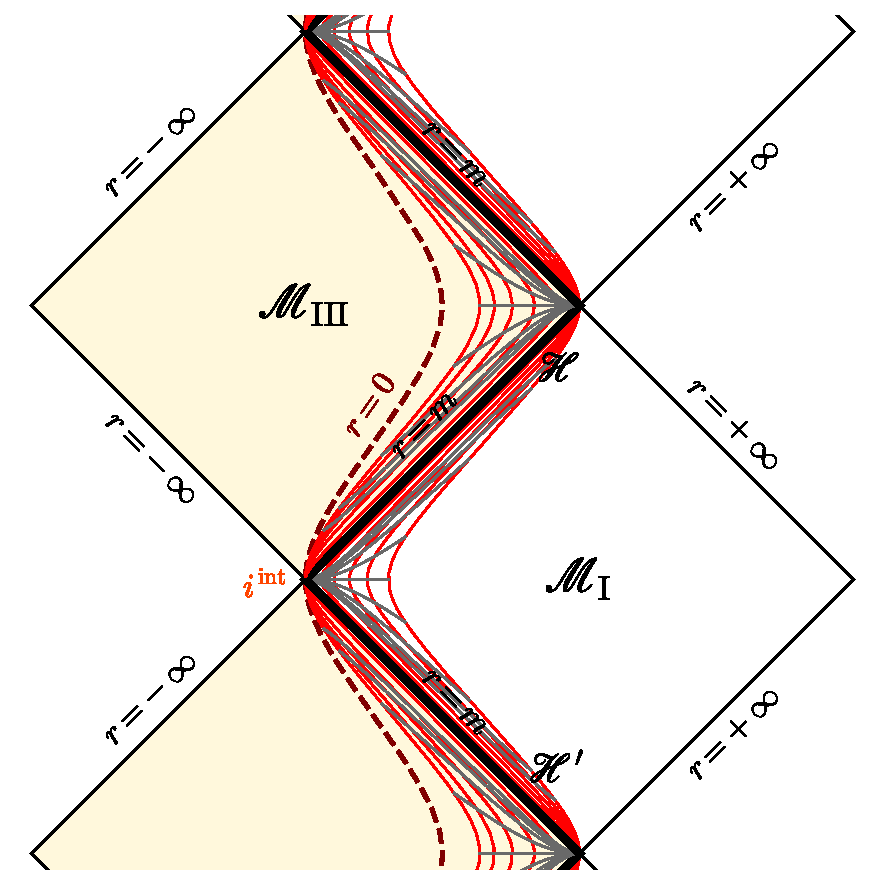
\includegraphics[width=\textwidth]{exk_NH_region.pdf} \\[1ex]
\
\end{minipage}
\hfill
\begin{minipage}[c]{0.35\textwidth}
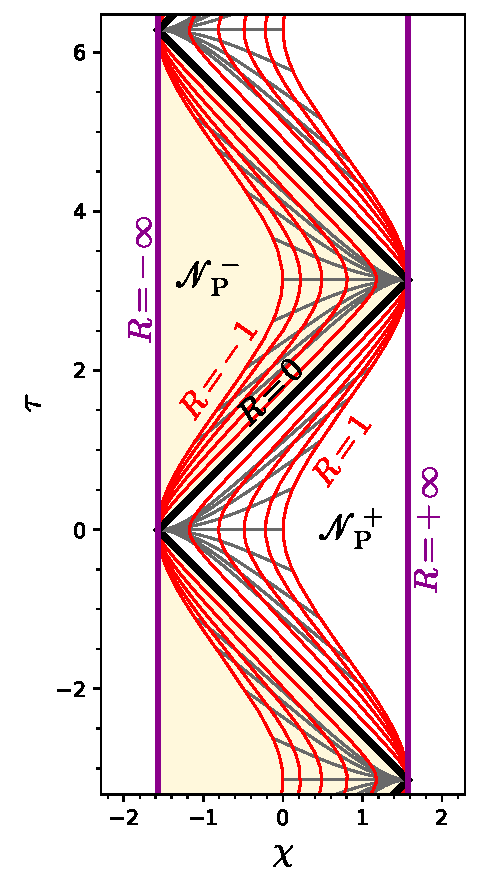
\includegraphics[width=\textwidth]{exk_NHEK_spacetime.pdf}
\end{minipage}
\caption[]{\label{f:exk:compar_Kerr_NHEK} \footnotesize
2-dimensional views of the extremal Kerr spacetime  $(\M, \w{g})$ (left) and of
the NHEK spacetime $(\mathscr{N},\w{h})$ (right). The left figure is a zoom
on the $(\M_{\rm I}^{(0)}, \M_{\rm III}^{(0)})$ part of
the Carter-Penrose diagram
shown in Fig.~\ref{f:exk:CPdiag_maximal}.
The right figure is a ``compactified'' view of $\mathscr{N}$
based on the coordinates $(\tau,\chi)$. The near-horizon region in
the Kerr spacetime is visualized by means of red curves, which
are curves (actually hypersurfaces) of constant $r$,
ranging from $r=m/2$ to $r=3m/2$, i.e. within $\Delta r = m/2$ of the horizon value $r=m$.
The $r$-increment between two nearby curves is $\delta r = m/10$.
Grey curves represents hypersurfaces of constant Boyer-Lindquist coordinate $t$
in the near horizon region, with $t$ varying by steps of $\delta t = 2m$
in the range $[-8m, 8m]$. Each of these constant-$r$ or constant-$t$ curves is mapped
to the NHEK spacetime (right figure) by means of the transformation
(\ref{e:exk:R_T_Phi_BL}) with $\veps=1/2$, giving birth to constant-$R$
curves ranging from $R=-1$ to $R=1$ (red curves) and to constant-$T$
curves ranging from $T=-2$ to $T=2$ (grey curves).
\textsl{[Figures generated by the notebooks \ref{s:sam:Kerr_extremal_extended} (left)
and \ref{s:sam:NEHK_spacetime} (right)]}
}
\end{figure}



\subsubsection{``Conformal'' coordinates}

The range of the coordinate $y$ is the whole of $\R$. For pictural purposes (e.g. drawing
Carter-Penrose-like diagrams), it
would be convenient to have instead a coordinate spanning some finite range.
As in the AdS$_4$ case presented in Example~\ref{x:neh:AdS}
of Chap.~\ref{s:neh}, it is quite natural to introduce
\be
    \chi := \arctan y \quad\iff\quad y =: \tan\chi
\ee
so that\footnote{In Example~\ref{x:neh:AdS}, the range of $\chi$ was only
$(0,\pi/2)$
because $r = \tan\chi \ge 0$ in AdS$_4$, while here $y=\tan\chi$ spans the whole of $\R$.}
$\chi\in (-\pi/2, \pi/2)$.
The relation (\ref{e:exk:def_global_NHEK}) to the Bardeen-Horowitz coordinates $(T,R,\theta,\Phi)$
can be then rewritten as
\be \label{e:exk:T_R_Phi_tau_chi_psi}
    \left\{ \begin{array}{l}
    T = \frac{\sin\tau}{\cos\tau + \sin\chi} \\[1ex]
    R = \frac{\cos\tau + \sin\chi}{\cos\chi} \\[1ex]
    \theta = \theta\\[1ex]
    \Phi = \psi + \ln\left|\frac{\cos(\tau - \chi)}{\sin\tau + \cos\chi} \right|
    \end{array}\right.
    \iff
    \left\{ \begin{array}{l}
    \tau = \arctantwo\left(2 T R^2, R^2 - T^2 R^2 + 1\right) + \pi H(-R)\\[1ex]
    \chi = \arctan \left(\frac{(1 + T^2)R^2 - 1}{2R}  \right)\\[1ex]
    \theta = \theta\\[1ex]
    \psi = \Phi - \ln\left(
      \frac{(1 - TR)^2 + R^2}{\sqrt{[(1 + T^2)R^2 - 1]^2 + 4R^2}} \right) ,
    \end{array}\right.
\ee
These transformations can be used to map
the Boyer-Lindquist domain $\M_{\rm BL}$
of Kerr spacetime to the region $- \pi/2 < \tau + \chi< 3\pi/2$
of the NHEK spacetime $\mathscr{N}$, as illustrated in Fig.~\ref{f:exk:compar_Kerr_NHEK}.
This assumes a fixed value of $\veps > 0$ in Eqs.~(\ref{e:exk:def_R_T_Phi})-(\ref{e:exk:R_T_Phi_BL}),
so that $(T,R,\th,\Phi)$ constitute a regular coordinate system on
$\M_{\rm BL}=\M_{\rm I}\cup \M_{\rm III}$.
More precisely,
$\M_{\rm I}$, where $R>0$, is mapped to the subregion $\mathscr{N}_{\rm P}^+$
defined by $-\chi - \pi/2 < \tau < \chi + \pi/2$, which
implies $\cos\tau + \sin\chi > 0$ and hence $R>0$ via (\ref{e:exk:T_R_Phi_tau_chi_psi}),
since $\cos\chi>0$ for $\chi\in(-\pi/2,\pi/2)$.
On the other hand, $\M_{\rm III}$, where $R<0$, is mapped to the subregion
$\mathscr{N}_{\rm P}^-$ defined by $\chi + \pi/2 < \tau < -\chi + 3\pi/2$,
which implies $\cos\tau + \sin\chi < 0$ and hence $R<0$ via (\ref{e:exk:T_R_Phi_tau_chi_psi}).
In both $\mathscr{N}_{\rm P}^+$
and $\mathscr{N}_{\rm P}^-$, the coordinate $T$ spans the whole of $\R$.
We shall call each of the regions $\mathscr{N}_{\rm P}^+$
and $\mathscr{N}_{\rm P}^-$  a \defin{Poincaré patch of NHEK spacetime}\index{Poincaré!patch!of NHEK}.
They appear as the interiors of triangles having one vertical edge at the NHEK
boundary in Fig.~\ref{f:exk:compar_Kerr_NHEK}. Note the similarity\footnote{In
Fig.~\ref{f:neh:AdS_example}, the Poincaré patch (where $u>0$)
has its vertical edge on the left, while in Fig.~\ref{f:exk:compar_Kerr_NHEK},
$\mathscr{N}_{\rm P}^+$ (where $R>0$) has its vertical edge on the right, but this results simply
from a distinct convention in choosing $\chi$.}
with the Poincaré patch in AdS$_4$ spacetime plotted in Fig.~\ref{f:neh:AdS_example}.

The NHEK metric components with respect to the coordinates
$(\tau,\chi,\th,\psi)$ are easily deduced from
(\ref{e:exk:global_NEHK_metric}):
\be
    \encadre{
    \w{h} =
    m^2 (1 + \cos^2\th) \left[
    \frac{1}{\cos^2\chi} \left( - \dd \tau^2 + \dd \chi^2 \right)
    + \dd\th^2 + \frac{4 \sin^2\th}{(1 + \cos^2\th)^2}
    \left( \dd\psi + \tan\chi\,  \dd \tau\right)^2 \right]
    } .
\ee
Note the factor $1/\cos^2\chi$ in front of the
$- \dd \tau^2 + \dd \chi^2$ term, which is analogous to the conformal factor
$1/\cos^2\chi$ of the AdS$_4$ metric in Eq.~(\ref{e:neh:metrix_AdS_conformal}),
except that in the present case, $1/\cos^2\chi$ does not factor all the
metric, so that it cannot be considered as a proper conformal factor. Since $\cos\chi$ never vanishes
for $\chi\in(-\pi/2, \pi/2)$,
the factor $1/\cos^2\chi$ is regular in all $\mathscr{N}$. It simply blows up
at the ``boundaries'' $\chi\to \pm \pi/2$ of $\mathscr{N}$,
which correspond to $y\to \pm\infty$ and to $R\to \pm\infty$ in the Poincaré patches
$\mathscr{N}_{\rm P}^+$ and $\mathscr{N}_{\rm P}^-$.

One can provide a pictoral view of $\w{h}$ being the ``near-horizon limit'' of $\w{g}$ as follows:

\begin{greybox}
The two red strips $r\in[m/2, 3m/2]$ and $R\in[-1, 1]$
in Fig.~\ref{f:exk:compar_Kerr_NHEK} have been drawn by setting
$\veps=1/2$ in the transformation (\ref{e:exk:R_T_Phi_BL}) linking the Boyer-Lindquist coordinates
$(t,r,\th,\ph)$ to the Bardeen-Horowitz ones $(T,R,\th,\Phi)$. Now, if one maintains
the red strip $R\in[-1, 1]$ in the NHEK spacetime unchanged and let $\veps$ decays to $0$,
the red strip in the extremal Kerr spacetime  shrinks to a more and more narrow strip
around the horizon. As $\veps\to 0$, this narrow strip, endowed with the Kerr metric $\w{g}$, tends
to be isometric to the fixed NHEK strip $R\in[-1, 1]$ endowed with the metric $\w{h}$.
\end{greybox}

\begin{remark}
While the extremal Kerr spacetime and the NHEK one are similar in the
near-horizon region, it is clear on Fig.~\ref{f:exk:compar_Kerr_NHEK} that they
have very different asymptotics for $r\to \pm \infty$ and $R\to \pm \infty$.
\end{remark}

\subsection{NHEK symmetries}

Given the similarities with the AdS spacetime, which is a maximally symmetric spacetime\footnote{A spacetime of dimension $n$
is said to be \defin{maximally symmetric}\index{maximally symmetric} if, and only if,
its group of isometries has the maximum possible dimension, which is $n(n+1)/2$.
It is equivalent to say that there are $n(n+1)/2$ linearly independent Killing vector fields
when considering only linear combinations with constant coefficients.
For $n=4$, one has $n(n+1)/2=10$, which, among others,
is the dimension of the Poincaré group\index{Poincaré!group} (isometries of Minkowski spacetime).
The group of isometries of AdS$_n$ is the pseudo-orthogonal group $\mathrm{O}(2, n-1)$,
the dimension of which is exactly $n(n+1)/2$ (cf. e.g. Ref.~\cite{ONeil83}).},
it should come as no surprise that the NHEK spacetime $(\mathscr{N},\w{h})$
has more symmetries than the extremal Kerr spacetime $(\M,\w{g})$. First of all, it is
obvious on the expression (\ref{e:exk:NEHK_metric}) of $\w{h}$
in Bardeen-Horowitz coordinates that $T$ and $\Phi$ are ignorable coordinates,
so that the two vector fields
\be \label{e:exk:xi1_eta}
   \w{\xi}_1 := \wpar_T =   \frac{2m}{\veps} \wpar_t + \frac{1}{\veps} \wpar_\ph
   \qand
   \w{\eta} = \wpar_\Phi = \wpar_\ph = \wpar_\psi
\ee
are two Killing vectors of $\w{h}$. In the above equation, the second expression of $\w{\xi}_1$
is that in the Boyer-Lindquist coordinate frame and
follows directly from the transformation law (\ref{e:exk:def_R_T_Phi}).
In particular, note that $\w{\xi}_1$ is distinct from the Killing vector
$\w{\xi} = \wpar_t$ of the Kerr metric $\w{g}$. It is rather connected
to the horizon-generating Killing vector $\w{\chi}$ defined by
Eq.~(\ref{e:exk:def_chi}):
\be
    \w{\xi}_1 = \frac{2 m}{\veps} \w{\chi} .
\ee
Besides, in Eq.~(\ref{e:exk:xi1_eta}),
the vector field $\wpar_\Phi$ is identical
to the Killing vector field $\w{\eta} = \wpar_\ph$ of the Kerr metric $\w{g}$
as a consequence of the transformation law (\ref{e:exk:def_R_T_Phi}). Similarly,
the transformation law (\ref{e:exk:def_global_NHEK}) implies that
$\w{\eta} = \wpar_\psi$.

A third symmetry apparent on the metric components (\ref{e:exk:NEHK_metric})
is the invariance under the transformation $(T,R) \mapsto (\alpha T,\, R/\alpha)$,
for any $\alpha > 0$.
Such transformations, which are called \defin{squeeze mappings}\index{squeeze mapping}, or
\defin{hyperbolic rotations}\index{hyperbolic!rotation} of the $(T,R)$ plane, form
a 1-parameter group action, whose generator
$\w{\xi}_2$ is given by formula~(\ref{e:neh:xi_dxdt}) with $t = \lambda := \alpha - 1$ (so that the
identity element is for $\lambda=0$). By considering an infinitesimal transformation
of parameter $\D\lambda$, formula~(\ref{e:neh:xi_dxdt}) leads to the components
$\xi_2^T = [(1 + \D\lambda) T - T]/\D\lambda = T$ and
$\xi_2^R = [(1 - \D\lambda) R - R]/\D\lambda = - R$.
Hence the Killing vector field
\be \label{e:exk:xi2}
    \w{\xi}_2 = T \, \wpar_T - R \, \wpar_R
      = t \, \wpar_t + (m - r) \, \wpar_r + \frac{t}{2m}\, \wpar_\ph .
\ee
The second expression stems from the transformation law  (\ref{e:exk:def_R_T_Phi})
and expresses $\w{\xi}_2$ in terms of the Boyer-Lindquist coordinate frame.
We note that this expression is independent of $\veps$,
contrary to the Boyer-Lindquist expression of $\w{\xi}_1$.

Finally, a fourth Killing vector of $\w{h}$ shows up clearly on the
components (\ref{e:exk:global_NEHK_metric})
with respect to the global NHEK coordinates $(\tau,y,\th,\psi)$, since these components
are independent of $\tau$. Hence $\wpar_\tau$ is a Killing vector of
$\w{h}$. In what follows, we will use instead the linear combination\footnote{Let us recall that
a linear combination with constant coefficients of Killing vectors is a Killing vector.}
\be
    \w{\xi}_3 := \wpar_\tau - \frac{1}{2}\, \w{\xi}_1,
\ee
since it has slightly simpler
components with respect to Bardeen-Horowitz coordinates. Given the
transformation law (\ref{e:exk:def_global_NHEK}), we get (cf. the notebook~\ref{s:sam:NEHK})
\be \label{e:exk:xi3}
    \w{\xi}_3 = \frac{1}{2}\left( T^2+ \frac{1}{R^2} \right) \wpar_T
    - RT \, \wpar_R - \frac{1}{R} \wpar_\Phi .
\ee
The Boyer-Lindquist expression of $\w{\xi}_3$ is found via the transformation
law (\ref{e:exk:def_R_T_Phi})-(\ref{e:exk:R_T_Phi_BL}):
\be
    \w{\xi}_3 = \veps \left\{ \left[ \frac{t^2}{4m} + \frac{m^3}{(r - m)^2} \right]
    \wpar_t + \frac{t(m - r)}{2m} \wpar_r
    + \frac{1}{2} \left[ \frac{t^2}{4m^2} + \frac{m(3m - 2r)}{(r - m)^2} \right]
    \wpar_\ph \right\} .
\ee

We have thus four Killing vectors of the NEHK metric $\w{h}$:
$\w{\eta}$, $\w{\xi}_1$, $\w{\xi}_2$ and  $\w{\xi}_3$.
Since none of them is a linear combination with constant coefficients
of the three others, the isometry group $G$
generated by these Killing vectors is 4-dimensional. This is
2 dimensions more than
the isometry group of Kerr spacetime, which is $\mathbb{R}\times\mathrm{U}(1)$.
In order to fully characterize $G$,
let us determine its Lie algebra\index{Lie!algebra} by evaluating
the commutator\footnote{The definition of the commutator
of two vector fields is recalled in Appendix~\ref{s:bas} [cf. Eq.~(\ref{e:bas:def_commutator})].} of each pair
of the four generators $\w{\eta}$, $\w{\xi}_1$, $\w{\xi}_2$ and  $\w{\xi}_3$.
We get (cf. the notebook~\ref{s:sam:NEHK})
\be \label{e:exk:commut_eta}
    [\w{\eta}, \w{\xi}_1] = 0,\quad
    [\w{\eta}, \w{\xi}_2] = 0,\quad
    [\w{\eta}, \w{\xi}_3] = 0
\ee
and
\be \label{e:exk:commut_sl2}
    [\w{\xi}_2, \w{\xi}_1] = - \w{\xi}_1, \quad
    [\w{\xi}_2, \w{\xi}_3] = \w{\xi}_3, \quad
    [\w{\xi}_1, \w{\xi}_3] = \w{\xi}_2 .
\ee
Equation~(\ref{e:exk:commut_eta}) shows that $\w{\eta}$ commutes with all the
other generators of $G$. Since $\w{\eta}$ is the
generator of the axisymmetry group $\mathrm{U}(1)$, we may write
$G = G_3\times \mathrm{U}(1)$, where $G_3$ is a
3-dimensional Lie group, generated by $\w{\xi}_1$, $\w{\xi}_2$ and
$\w{\xi}_3$. The commutation relations (\ref{e:exk:commut_sl2})
show\footnote{More precisely, in the representation of
$\mathfrak{sl}(2,\R)$ by the algebra of $2\times 2$ real matrices with zero
trace, a standard basis is
$E = \scriptscriptstyle \left( \begin{array}{cc}0 & 1\\[-1ex] 0 & 0 \end{array}\right)$,
$F = \scriptscriptstyle \left( \begin{array}{cc}0 & 0\\[-1ex] 1 & 0 \end{array}\right)$,
$H = \scriptscriptstyle \left( \begin{array}{cc}1 & 0\\[-1ex] 0 & -1 \end{array}\right)$.
This basis has the following commutation relations:
$[H, E] = 2E$, $[H, F] = - 2F$ and $[E,F] = H$. One recovers the last ones
from (\ref{e:exk:commut_sl2})
by identityfying $\w{\xi}_1$ with $F/\sqrt{2}$, $\w{\xi}_2$ with $H/2$
and  $\w{\xi}_3$ with $-E/\sqrt{2}$.}
that the Lie algebra of $G_3$ is the special
linear algebra $\mathfrak{sl}(2,\R)$.
At this stage, $G_3$ can be one of the following three
Lie groups: $\mathrm{SL}(2,\R)$, $\mathrm{PSL}(2,\R) = \mathrm{SL}(2,\R)/\mathbb{Z}_2$
or $\overline{\mathrm{SL}(2,\R)}$
(the universal covering group of $\mathrm{SL}(2, \mathbb{R})$).
It cannot be $\mathrm{PSL}(2,\R)$ because, as it appears clearly on (\ref{e:exk:NEHK_metric}),
the transformation $(T,R) \mapsto (-T,-R)$ is an element of $G_3$ and, in $\mathrm{PSL}(2,\R)$, this element would be identified with the identity
due to the quotient by $\mathbb{Z}_2 = \{\mathrm{Id}, -\mathrm{Id}\}$, where $\mathrm{Id}$
is the identity element.
$G_3$ is actually the
special linear group $\mathrm{SL}(2,\R)$. We conclude:
\begin{prop}[isometry group of NEHK spacetime]
The isometry group
of the NEHK spacetime is
\be \label{e:exk:NHEK_isometry_group}
    \encadre{ G = \mathrm{SL}(2,\R)\times \mathrm{U}(1) } ,
\ee
with $\mathrm{U}(1)$ generated by the axisymmetry Killing vector $\w{\eta}$ and
$\mathrm{SL}(2,\R)$ generated by the three Killing vectors $\w{\xi}_1$, $\w{\xi}_2$ and
$\w{\xi}_3$ given by Eqs.~(\ref{e:exk:xi1_eta}), (\ref{e:exk:xi2}) and (\ref{e:exk:xi3}).
\end{prop}

This property is often phrased as follows: the near-horizon region of the extremal
Kerr spacetime (the extremal Kerr throat) has some \emph{emergent symmetries}, i.e. it has
more symmetries than the extremal Kerr spacetime itself.
Let us stress that no such thing occurs for non-extremal Kerr black holes.

\begin{remark}
$\mathrm{SL}(2,\R)$ is isomorphic to the spin group $\mathrm{Spin}(2,1)$,
which is the isometry group of the 2-dimensional anti-de Sitter spacetime (AdS$_2$).
The spin group $\mathrm{Spin}(2,1)$ is the double cover of the pseudo-orthogonal group $\mathrm{SO}(2,1)$, the latter being the isometry group of the ``time-cyclic'' 2-dimensional
anti-de Sitter spacetime, i.e. the quadric surface $X^2 - U^2 - V^2 = -1$ in
$\mathbb{R}^3$ endowed with the flat metric $-\dd U^2 - \dd V^2 + \dd X^2$.
\end{remark}

\begin{remark}
Having an enhanced symmetry group near the horizon is not specific to the
extremal Kerr black hole;
this is actually a generic feature, which occurs near \emph{degenerate} Killing horizons
\cite{KunduL13,Compe17}.
Pure geometric arguments suffice to show that a degenerate Killing horizon
associated with some Killing vector $\w{\xi}_1$ has necessarily a near-horizon geometry
endowed with a second Killing vector, which is similar to $\w{\xi}_2$ \cite{KunduL13}.
Axisymmetry provides the third Killing vector $\w{\eta}$ and the Einstein equation
leads to the existence of the fourth Killing vector $\w{\xi}_3$
\cite{KunduLR07}.
\end{remark}

\begin{hist} \label{h:exk:NHEK_metric}
The NHEK metric $\w{h}$ has been first exhibited by Brandon Carter\index[pers]{Carter, B.} in 1973 \cite{Carte73a}:
compare Eq.~(5.63) of Ref.~\cite{Carte73a} (with $Q=P=0$) with Eq.~(\ref{e:exk:NEHK_metric}),
taking into account the change of notations $(\tau,\lambda,\varphi) \leftrightarrow (T,-R,\Phi)$.
Actually the NHEK metric was found by Carter when searching for the most general stationary
and axisymmetric solutions of the source-free Einstein-Maxwell equations (cf. Sec.~\ref{e:fra:electrovacuum}), in order to get
the Kerr-Newman\index{Kerr-Newman metric} solution. The latter appeared then as the generic case and NHEK-like metrics as
special cases. The limit $Q=P=0$ of Carter's metric (5.63) corresponds to the case
of vanishing electric charge $Q$ and magnetic monopole $P$, so that it is a solution
of the vacuum Einstein equation  [Eq.~(\ref{e:exk:Ricci_h_zero}) above].
Carter stated that the metric $\w{h}$ has a
4-dimensional isometry group and that the hypersurfaces of constant $\th$ are
homogeneous and partially isotropic.
Even if he did not get $\w{h}$ by some near-horizon limit process,
Carter stressed that in the neighborhood of the extremal Kerr horizon,
the Kerr metric $\w{g}$ can
be approximated arbitrarily closely by $\w{h}$
(cf. Fig.~6.3 in Ref.~\cite{Carte73a}, which is similar to our Fig.~\ref{f:exk:compar_Kerr_NHEK}).
In the related case of the \emph{static} extremal black hole,
constituted by the (spherically symmetric)
Reissner-Nordström\index{Reissner-Nordström metric} solution
with electric charge equal to the mass ($Q = m$), Carter exhibited
a change of coordinates similar\footnote{Carter defined the near-horizon coordinates
$(\tau,\lambda)$ by $t = m^2 \tau$ and $r = \lambda + m$ and took the
near-horizon limit as $m\to +\infty$
(cf. the paragraph surrounding Eq.~(4.31) in Ref.~\cite{Carte73a});
this is equivalent to Eq.~(\ref{e:exk:def_R_T_Phi})
with $\veps = 1/m$.}
to that between Boyer-Lindquist coordinates
and Bardeen-Horowitz coordinates [Eq.~(\ref{e:exk:def_R_T_Phi})] and
he showed that the near-horizon limit brings
the Reissner-Nordström metric to the
\emph{Bertotti-Robinson\index{Bertotti-Robinson spacetime} metric}.
The latter is the product metric of $\mathrm{AdS}_2\times\SS^2$ and constitutes a static solution of
the source-free Einstein-Maxwell equations that is highly symmetric, having the 6-dimensional
group $\mathrm{SL}(2,\R)\times\mathrm{SO}(3)$ as isometry group (cf. e.g. Ref.~\cite{GarfiG11}).
The NHEK metric has been rediscovered by James Bardeen\index[pers]{Bardeen, J.M.} and Gary Horowitz\index[pers]{Horowitz, G.T.} in 1999 \cite{BardeH99}. They deduced it from the Boyer-Lindquist expression of the extremal Kerr metric by performing the change of coordinates\footnote{The coordinates actually used by
Bardeen and Horowitz were $\tilde{T} := 2m T$ and $\tilde{R} = m R$, denoted
respectively $t$ and $r$ by them.}  (\ref{e:exk:def_R_T_Phi})-(\ref{e:exk:R_T_Phi_BL}) and taking the limit $\veps\to 0$, as presented in
Sec.~\ref{s:exk:NHEK_metric}. In the same article~\cite{BardeH99},
Bardeen and Horowitz introduced
the global NHEK coordinates\footnote{$\psi$ is denoted by $\phi$ in Ref.~\cite{BardeH99}.}
$(\tau,y,\th,\psi)$ via the transformation (\ref{e:exk:def_global_NHEK})
and obtained expression (\ref{e:exk:global_NEHK_metric}) for $\w{h}$ [their Eq.~(2.9)]. They have
analyzed the global properties of the NHEK spacetime, in particular its geodesic completeness.
Bardeen and Horowitz have also shown that the NHEK isometry group is
$\mathrm{SL}(2,\R)\times \mathrm{U}(1)$ [Eq.~(\ref{e:exk:NHEK_isometry_group})]
and have given formulas (\ref{e:exk:xi1_eta}), (\ref{e:exk:xi2}) and (\ref{e:exk:xi3})
for the four Killing vectors $\w{\xi}_1$, $\w{\xi}_2$, $\w{\xi}_3$ and $\w{\eta}$
[their Eq.~(2.14)].
\end{hist}

\subsection{Applications}

The NHEK geometry is at the core of the so-called \emph{Kerr/CFT correspondence}\index{Kerr/CFT correspondence}, initiated by Monica Guica\index[pers]{Guica, M.}, Thomas Hartman\index[pers]{Hartman, T.}, Wei Song\index[pers]{Song, W.} and Andrew Strominger\index[pers]{Strominger, A.} in 2009 \cite{GuicaHSS09}, which conjectures that quantum gravity\index{quantum!gravity}
in the vicinity of the extremal Kerr horizon is dual to a two-dimensional
conformal field theory\index{conformal!field theory} (CFT)\index{CFT}
(see Ref.~\cite{Compe17} for a review of this topic).

Another domain of application of the NHEK geometry regards the computation
of signals emanating from the neighborhood
of an extremal Kerr black hole, either
electromagnetic ones (e.g. \cite{GrallLS18,CompeD20,KapecL20})
or gravitational-wave ones (e.g. \cite{CompeFHL18,GrallPW15}).

\section{Going further}

Apart from the principal null geodesics, we have not discussed the geodesics
of the extremal Kerr black hole in this chapter. Many of their properties
can be obtained by taking the limit $a\to m$ of the Kerr geodesics discussed
in Chaps.~\ref{s:gek} and \ref{s:gik}. The specific case of critical null
geodesics, delineating the black hole shadow, has been treated in Sec.~\ref{s:gik:shadow_extremal}
for $a=m$.
For an extensive study of geodesics close to the horizon, making use of the NHEK geometry,
see Refs.~\cite{KapecL20,CompeD20}.

We have not discussed at all the stability of extremal Kerr black holes.
The main result in this respect is the so-called \defin{Aretakis instability}\index{Aretakis instability}: Stefanos Aretakis\index[pers]{Aretakis, S.} has shown in 2012\footnote{The work \cite{Areta15} appeared
on arXiv in 2012, but was published in 2015.} that scalar perturbations
(solutions of the wave equation $\Box_{\w{g}} \Psi = 0$)
do not decay along the event horizon $\Hor$ of an extremal Kerr black hole
and even that second and higher derivatives of $\Psi$ blow
up along $\Hor$ \cite{Areta15}
(see also the monograph \cite{Areta18}). In a subsequent study \cite{Areta13},
Aretakis has shown that solutions of the non-linear wave equation $\Box_{\w{g}}\Psi = N(\Psi,\wnab\Psi)$, where  $N$ is a non-linear function,
blow up in a finite time along $\Hor$.
The Aretakis instability has been shown to be related to the
enhanced symmetry group of the NHEK geometry \cite{GrallZ18}.







